\documentclass[11pt,a4paper]{article}

\usepackage[spanish, es-nodecimaldot]{babel}
\usepackage[T1]{fontenc}
\usepackage[utf8]{inputenc}

% Math essentials
\usepackage{amsmath, amssymb}
\usepackage{bm}

% Units and hyperlinks
\usepackage{siunitx}
\sisetup{per-mode=symbol}

\usepackage{natbib}
\usepackage{graphicx}
\usepackage{lmodern}
\usepackage{caption}
\usepackage{subcaption}
\usepackage{float}
\usepackage{url}
\usepackage{titlepic}
\usepackage{listings}
\usepackage{nameref}
\usepackage{xcolor}
\usepackage{array}
\setlength{\marginparwidth}{2cm}
\usepackage{todonotes}
\usepackage{datetime}
\usepackage{parskip}
\usepackage{hyperref}

% ------- Macros definidas en este documento -------
\newcommand{\vect}[1]{\bm{#1}}       % vectores en negrita cursiva
\newcommand{\mat}[1]{\mathbf{#1}}    % matrices en negrita recta
\newcommand{\trans}{\mathsf{T}}      % traspuesta, usar como ^{\trans}

\newcommand{\skewsym}[1]{\left[#1\right]_\times}

\newcommand{\SkewFrom}[3]{%
    \begin{bmatrix}
        \phantom{-}0   & -#3            & \phantom{-}#2  \\
        \phantom{-}#3  & \phantom{-}0   & -#1 \\
        -#2            & \phantom{-}#1  & \phantom{-}0
        \end{bmatrix}
}

\newcommand{\frameR}{\mathcal{R}}
\newcommand{\ejeXR}{X_{\frameR}}
\newcommand{\ejeYR}{Y_{\frameR}}

\newcommand{\frameB}{\mathcal{B}}
\newcommand{\ejeXB}{X_{\frameB}}
\newcommand{\ejeYB}{Y_{\frameB}}

\newcommand{\frameBi}{\mathcal{B}_i}
\newcommand{\ejeXBi}{X_{\frameBi}}
\newcommand{\ejeYBi}{Y_{\frameBi}}

\newcommand{\frameBZero}{\mathcal{B}_0}
\newcommand{\frameBNMinusOne}{\mathcal{B}_{N-1}}

\newcommand{\frameW}{\mathcal{W}}
\newcommand{\ejeXW}{X_{\frameW}}
\newcommand{\ejeYW}{Y_{\frameW}}

\newcommand{\frameWi}{\mathcal{W}_i}
\newcommand{\ejeXWi}{X_{\frameWi}}
\newcommand{\ejeYWi}{Y_{\frameWi}}

\title{Cinemática de robots terrestres: Un marco generalizado para la cinemática directa e inversa de robots terrestres con ruedas}
\author{Juan Francisco Rascón Crespo}
\date{\today}

\setcounter{secnumdepth}{2}
\setcounter{tocdepth}{2}

\begin{document}
\maketitle

\begin{abstract}
    Este documento presenta un desarrollo analítico riguroso de la cinemática directa e inversa para robots terrestres con ruedas. A partir de la definición de un sistema de coordenadas base invariante para cada rueda, se formula un sistema de ecuaciones matriciales que relaciona las velocidades individuales con el estado de movimiento del chasis. Dado que las plataformas con múltiples ruedas generan habitualmente sistemas sobredeterminados, se aborda su resolución óptima mediante el método de mínimos cuadrados y la pseudoinversa de Moore-Penrose. El texto pone un énfasis fundamental en la implementación en software y la estabilidad numérica, justificando detalladamente el uso de la Descomposición en Valores Singulares (SVD) para eludir las inestabilidades algebraicas. Asimismo, se introduce el análisis del número de condición (\(\kappa\)) como herramienta diagnóstica crítica para distinguir entre la robustez computacional del algoritmo y la viabilidad física del diseño mecánico. Finalmente, este marco teórico generalizado se aplica a la formulación y resolución cinemática de diversas topologías estándar en la robótica móvil, abarcando desde sistemas de tracción diferencial y dirección Ackermann, hasta plataformas omnidireccionales con ruedas Mecanum y configuraciones \textit{swerve drive}.
\end{abstract}

\section{Restricciones de movimiento impuestas por las ruedas}

En un robot terrestre, las ruedas imponen restricciones de movimiento. En ruedas convencionales, tanto orientables como no orientables, la rueda al girar sobre su eje de rotación se desplaza describiendo una trayectoria rectilínea en una determinada dirección que se denomina \textbf{dirección de rodadura}.

En las ruedas convencionales no orientables, la dirección de rodadura es fija, siempre apunta en la misma dirección, dado que la rueda no puede cambiar de orientación con respecto al chasis. En las ruedas convencionales orientables, primero la rueda se orienta hacia la dirección de rodadura deseada (pivotando sobre su eje vertical) y luego gira sobre su eje de rotación para desplazarse en esa dirección.

Tanto las ruedas convencionales orientables como las no orientables no pueden desplazarse en la dirección perpendicular a la dirección de rodadura, que es la dirección de su eje de rotación. Dicho de otra forma, la velocidad lateral de la rueda es nula, lo que se conoce como \textbf{restricción de no deslizamiento lateral}.

Por el contrario, en ruedas omnidireccionales y Mecanum/suecas, debido a la presencia de rodillos en su periferia que giran libremente, la dirección de rodadura de la rueda principal, aunque es fija y no cambia con el transcurrir del tiempo, no tiene por qué coincidir con la dirección de movimiento real de la rueda sobre el suelo. La rotación pasiva de los rodillos permite que la rueda tenga una velocidad lateral no nula (en dirección perpendicular a la dirección de rodadura; \textit{i.e.}, la dirección del eje de rotación de la rueda), eliminando la restricción de no deslizamiento lateral.

Estas restricciones se pueden expresar matemáticamente como ecuaciones que relacionan la velocidad lineal y angular de la rueda con la velocidad del robot. Estas ecuaciones son fundamentales para el diseño de controladores y planificadores de movimiento para robots terrestres, ya que determinan cómo el robot puede moverse en su entorno.

Apilando estas restricciones para cada rueda, se pueden derivar las ecuaciones de cinemática directa e inversa para diferentes configuraciones de robots terrestres, como robots con ruedas diferenciales, robots con ruedas omnidireccionales, y robots con ruedas activas orientables (swerve drive), entre otros.

En la figura \ref{fig:wheel-placement} se muestra el posicionamiento 2D de una rueda respecto al sistema de coordenadas (SC) del robot, \(\frameR\).
El término \(\alpha\) representa el ángulo que forma el eje \(\ejeXR\) con el vector de posición de la rueda, \(\vect{d}\), y por cómo se posiciona la rueda \textit{inicialmente}, es también el ángulo que forma el eje \(\ejeXR\) con el eje \(\ejeYW\). El eje \(\ejeXW\) es perpendicular al eje \(\ejeYW\) y su orientación con respecto al eje \(\ejeXR\) es \(\psi = \alpha - \frac{\pi}{2}\).
La magnitud del vector \(\vect{d}\), \(\left|\bm{d}\right| = d\),  es la distancia entre el SC \(\frameR\) y el SC \(\frameW\).

\begin{equation}
    \vect{d} = \begin{bmatrix} d\cos\alpha \\ d\sin\alpha \\ 0 \end{bmatrix}
\end{equation}

Nótese que para aliviar la notación, en este texto se omitirá el superíndice \({}^\frameR\), en los vectores y sus componentes que estén expresados con respecto del SC del robot, \(\frameR\). Así, en lugar de usar \({}^\frameR \vect{d}\), \({}^\frameR d_x\) y \({}^\frameR d_y\), se usará simplemente \(\vect{d}\), \(d_x\) y \(d_y\). Sin embargo, se mantendrá el superíndice en los vectores y componentes que estén expresados con respecto de otros SCs, como el SC base de la rueda, \(\frameB\), o el SC fijo a la rueda, \(\frameW\), para mayor claridad y evitar confusiones.

\begin{figure}[H]
    \centering
    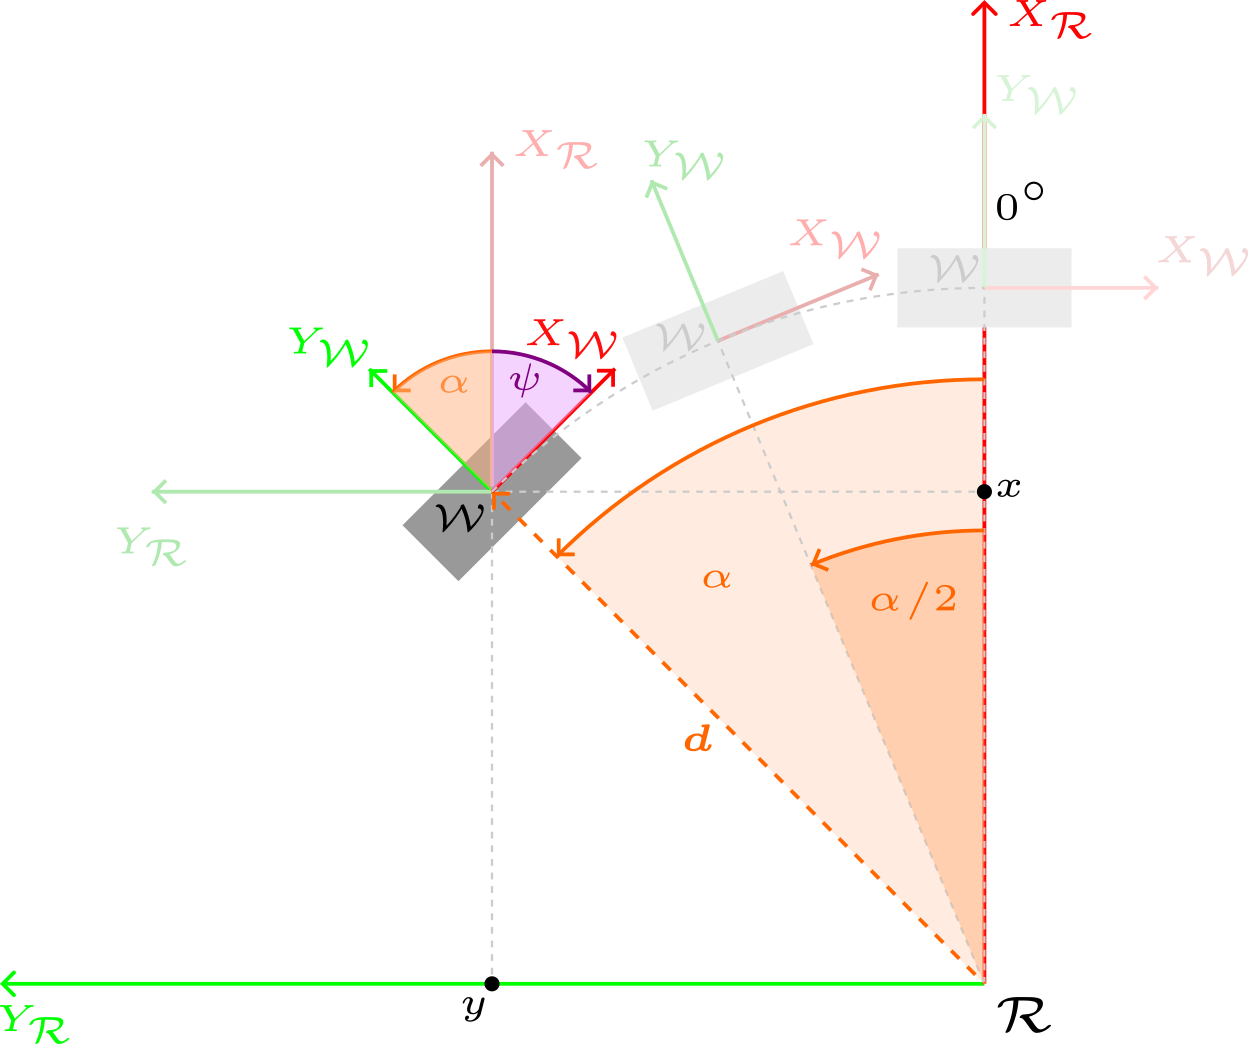
\includegraphics[width=1.0\linewidth]{images/wheel_placement.png}
    \caption{Posicionamiento 2D de una rueda respecto al SC del robot, \(\frameR\).}
    \label{fig:wheel-placement}
\end{figure}

A continuación, se considera un ángulo \(\beta\) que permite orientar la rueda de la manera deseada con respecto al SC \(\frameR\) (figura \ref{fig:wheel-orientation}), dando lugar al \textbf{SC base de la rueda}, \(\frameB\). El SC \(\frameB\) indica la ubicación (posición y orientación) de equilibrio/reposo/referencia de la rueda. El SC \(\frameB\) mantiene constante su posición y orientación en el tiempo con respecto del SC \(\frameR\). El SC \(\frameB\) se tiene en consideración en la formulación matemática porque resulta \textit{convenientemente adecuado} para definir la orientación de la rueda durante el movimiento del vehículo y aplicar restricciones de movimiento.

La orientación final de la rueda viene dada por el ángulo \(\psi\), formado entre el eje \(\ejeXR\) y el eje \(\ejeXB\).

\[
    \psi = \alpha + \beta - \frac{\pi}{2}
\]

y, para simplificar la notación se introduce el símbolo \(\phi\) como:

\[
    \phi = \alpha + \beta, \quad \psi = \phi - \frac{\pi}{2}
\]

\begin{figure}[H]
    \centering
    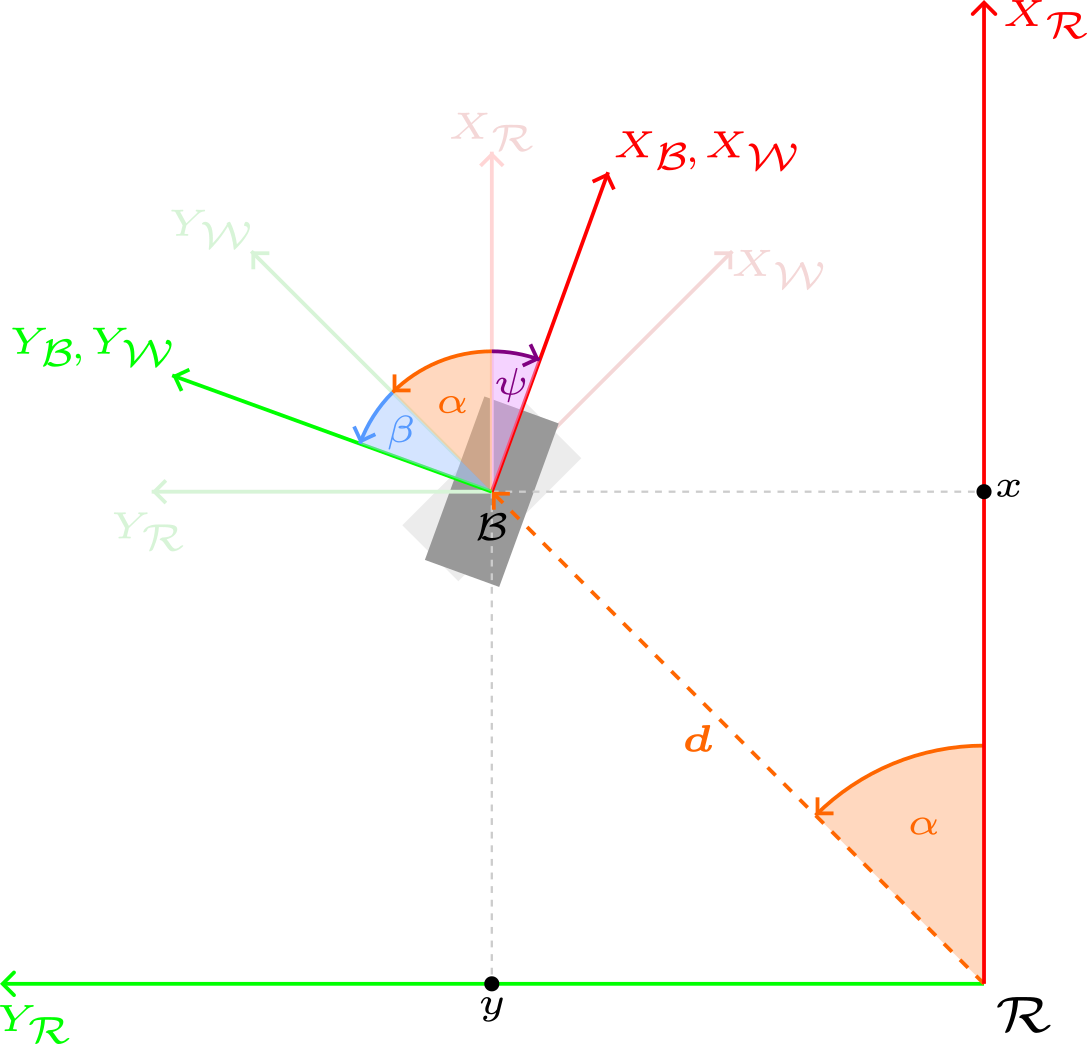
\includegraphics[width=1.0\linewidth]{images/wheel_orientation.png}
    \caption{Orientación de la rueda en la dirección de interés, mediante el ángulo \(\beta\).}
    \label{fig:wheel-orientation}
\end{figure}

En ruedas convencionales no orientables el eje \(\ejeXB\) y el eje \(\ejeXW\), eje X fijo a la rueda que indica la dirección de rodadura de la rueda, coinciden todo el tiempo. Solo por completitud, se menciona que en este tipo de ruedas el eje \(\ejeYB\) y el eje \(\ejeYW\), eje Y fijo a la rueda que indica la dirección de su eje de rotación, también coinciden todo el tiempo, obviamente.

En ruedas orientables, el SC \(\frameW\), fijo a la rueda, va cambiando su orientación, \(\theta\), respecto al SC \(\frameB\). Sólo cuando \(\theta=0\) ambos SCs coinciden. Ver figura \ref{fig:rolling-direction}.

\begin{figure}[H]
    \centering
    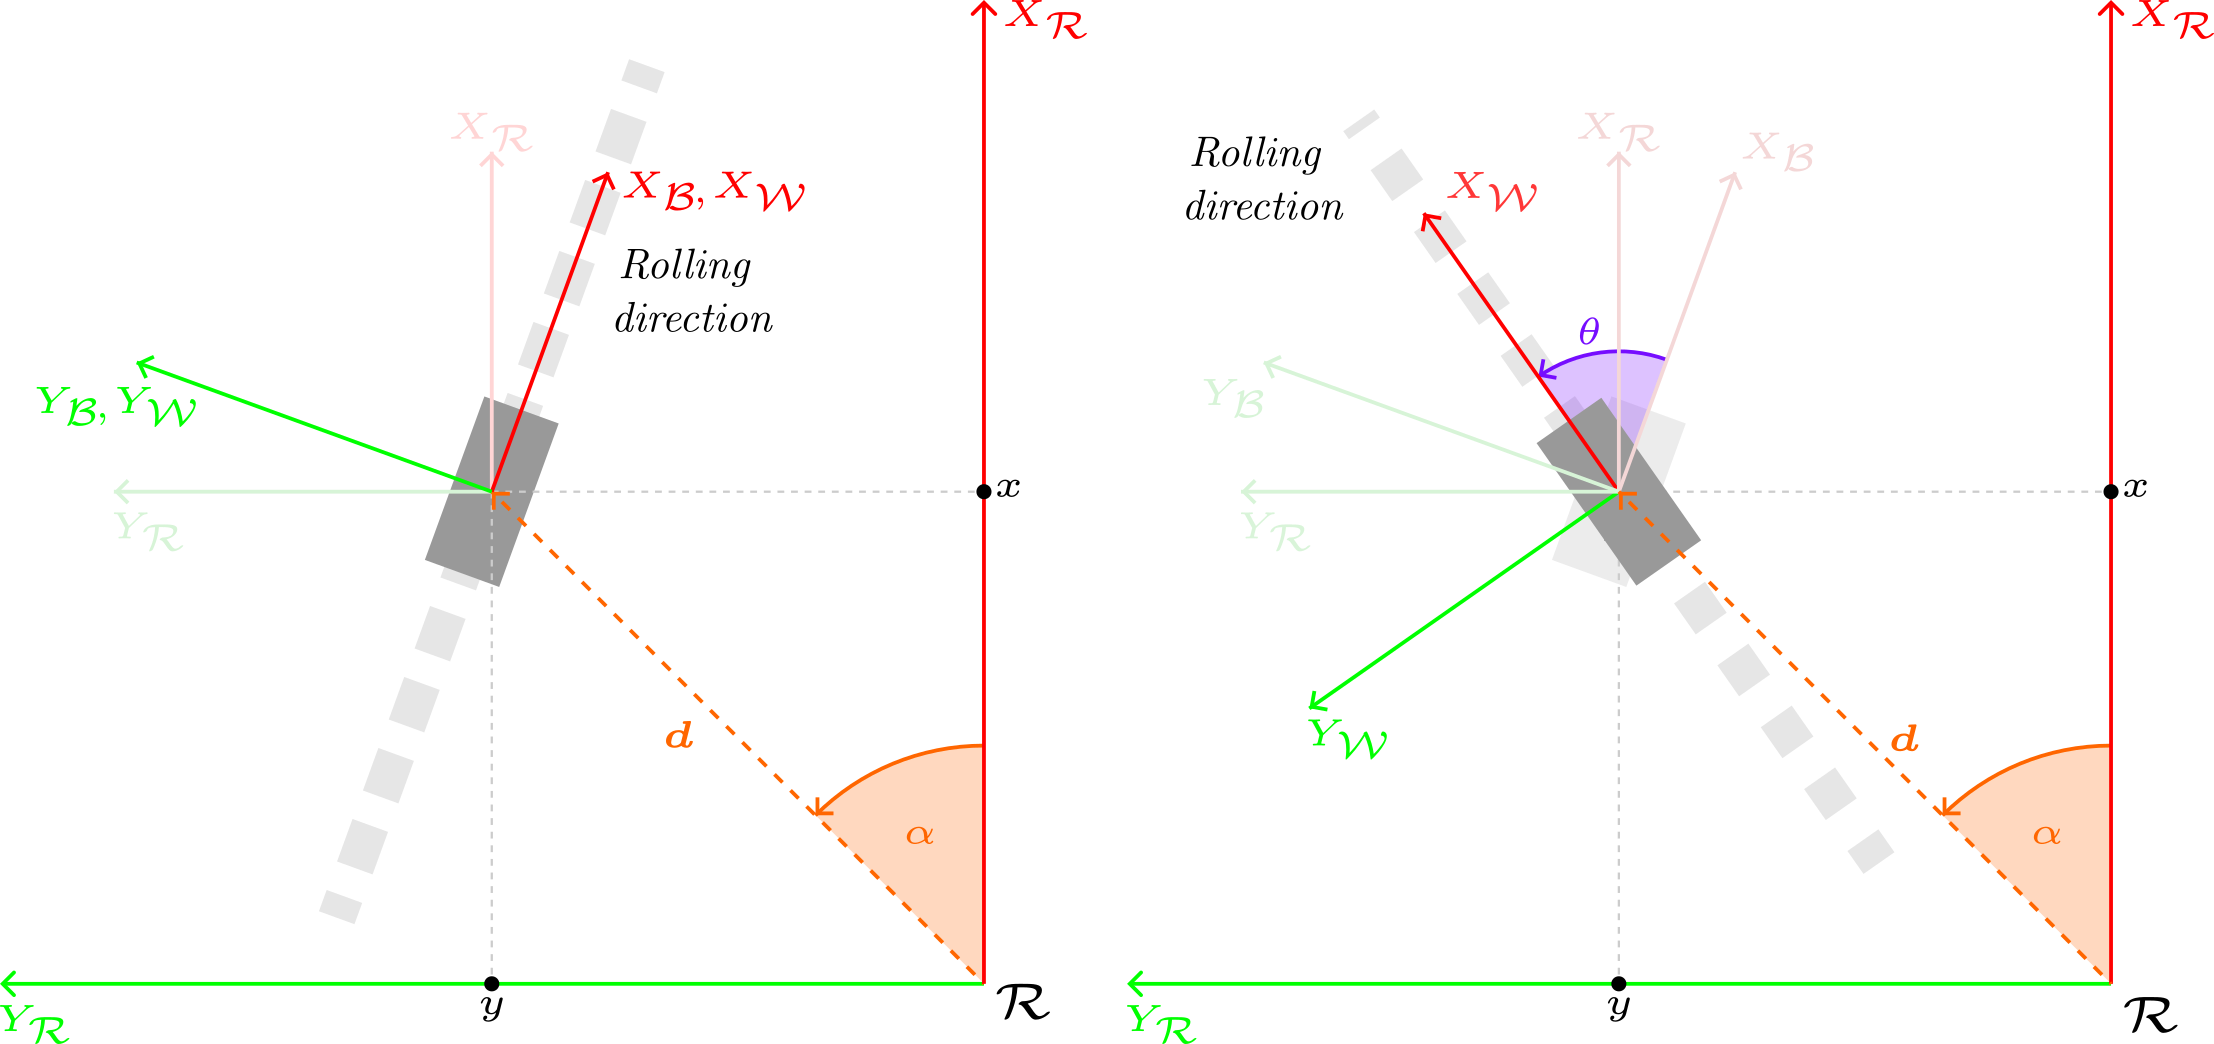
\includegraphics[width=1.0\linewidth]{images/rolling_direction.png}
    \caption{Izquierda: Rueda convencional no orientable. El SC \(\frameW\), fijo a la rueda, coincide todo el tiempo con el SC base de la rueda, \(\frameB\). La dirección de rodadura está indicada por la dirección del eje \(\ejeXW\) y en este caso es fija. Derecha: Rueda convencional orientable. El SC \(\frameW\), fijo a la rueda, va cambiando su orientación (\(\theta\)) respecto del SC base de la rueda, \(\frameB\). La dirección de rodadura está indicada por la dirección del eje \(\ejeXW\) y puede variar a lo largo del tiempo.}
    \label{fig:rolling-direction}
\end{figure}

La velocidad lineal de la base, expresada en el SC del robot, se denota como:

\begin{equation}
    \vect{V}_r = \begin{bmatrix} V_{r,x} \\ V_{r,y} \\ 0 \end{bmatrix}
    \label{eq:rigid-velocity}
\end{equation}

y se expresa en \si{\meter\per\second}.

De nuevo, nótese que para aliviar la notación, en este texto se omitirá el superíndice \({}^\frameR\), en los vectores y sus componentes que estén expresados con respecto del SC del robot, \(\frameR\). Así, en lugar de usar \({}^\frameR \vect{V}_r\), \({}^\frameR V_{r,x}\) y \({}^\frameR V_{r,y}\), se usará simplemente \(\vect{V}_r\) y \(V_{r,x}\), \(V_{r,y}\). Sin embargo, se mantendrá el superíndice en los vectores y componentes que estén expresados con respecto de otros SCs, como el SC base de la rueda, \(\frameB\), o el SC fijo a la rueda, \(\frameW\), para mayor claridad y evitar confusiones.

La velocidad angular de la base se denota como:

\begin{equation}
    \vect{\omega}_r = \begin{bmatrix} 0 \\ 0 \\ \omega_{r,z} \end{bmatrix}
    \label{eq:rigid-angular-velocity}
\end{equation}

y se expresa en \si{\radian\per\second}.

Un vez más, y por ser explícito en este texto, se omite el superíndice \({}^\frameR\) en los componentes de la velocidad angular que estén expresados con respecto del SC del robot, \(\frameR\). Así, en lugar de usar \({}^\frameR \vect{\omega}_r\) y \({}^\frameR \omega_{r,z}\), se usará simplemente \(\vect{\omega}_r\) y \(\omega_{r,z}\).

La velocidad lineal de cada rueda \(i\) expresada en el SC \(\frameR\) se denota como:

\begin{equation}
    \vect{V}_{i}  = \vect{V}_r + \vect{\omega}_r \times \vect{d}_{i}
    \label{eq:wheel-velocity}
\end{equation}

donde \(\vect{d}_{i}\) es el vector de posición de la rueda \(i\) respecto del SC \(\frameR\).

El producto vectorial \(\vect{\omega}_r \times \vect{d}_{i}\) puede escribirse como un producto matricial mediante el operador antisimétrico \(\skewsym{\cdot}\):

\begin{equation}
    \skewsym{\vect{\omega}_r} \triangleq
    \SkewFrom{\omega_{r,x}}{\omega_{r,y}}{\omega_{r,z}}
\end{equation}

\begin{equation}
    \begin{aligned}
        \vect{\omega}_r \times \vect{d}_{i} & = \skewsym{\vect{\omega}_r} \vect{d}_{i} =   \\
                                            & = \begin{bmatrix}
                                                    0            & -\omega_{r,z} & 0 \\
                                                    \omega_{r,z} & \phantom{-}0  & 0 \\
                                                    0            & \phantom{-}0  & 0
                                                \end{bmatrix} \begin{bmatrix}
                                                                  d_{i}\cos\alpha_i \\
                                                                  d_{i}\sin\alpha_i \\
                                                                  0
                                                              \end{bmatrix}           =    \\
                                            & = \begin{bmatrix}
                                                    -\omega_{r,z} d_{i} \sin\alpha_i           \\
                                                    \phantom{-}\omega_{r,z} d_{i} \cos\alpha_i \\
                                                    0
                                                \end{bmatrix}
    \end{aligned}
\end{equation}

\begin{equation}
    \begin{aligned}
        \vect{V}_{i} & = \vect{V}_r + \vect{\omega}_r \times \vect{d}_i = \\
                     & = \begin{bmatrix}
                             V_{r,x} - \omega_{r,z} d_{i} \sin\alpha_i \\
                             V_{r,y} + \omega_{r,z} d_{i} \cos\alpha_i
                         \end{bmatrix} =        \\
                     & = \begin{bmatrix}
                             1 & 0 & -d_{i} \sin\alpha_i           \\
                             0 & 1 & \phantom{-}d_{i} \cos\alpha_i
                         \end{bmatrix} \begin{bmatrix}
                                           V_{r,x} \\
                                           V_{r,y} \\
                                           \omega_{r,z}
                                       \end{bmatrix}
    \end{aligned}
    \label{eq:wheel-velocity-frameR}
\end{equation}

Para aplicar restricciones físicas al movimiento de cada rueda \(i\) primero se debe expresar su velocidad en su SC base, \(\frameBi\), \({}^{\frameBi} \vect{V}_{i}\).

\begin{equation}
    {}^{\frameBi} \vect{V}_{i} = \begin{bmatrix}
        {}^{\frameBi}V_{i,x} \\
        {}^{\frameBi}V_{i,y}
    \end{bmatrix} = {}^{\frameBi} R(\psi_i)_{\frameR} \vect{V}_{i}
    \label{eq:wheel-velocity-frameBi}
\end{equation}

donde la matriz de rotación \({}^{\frameBi}  R(\psi_i)_{\frameR}\) representa la orientación del SC \(\frameR\) en el SC \(\frameBi\), y se usa para convertir vectores expresados en el SC \(\frameR\) al SC \(\frameBi\).

\begin{figure}[H]
    \centering
    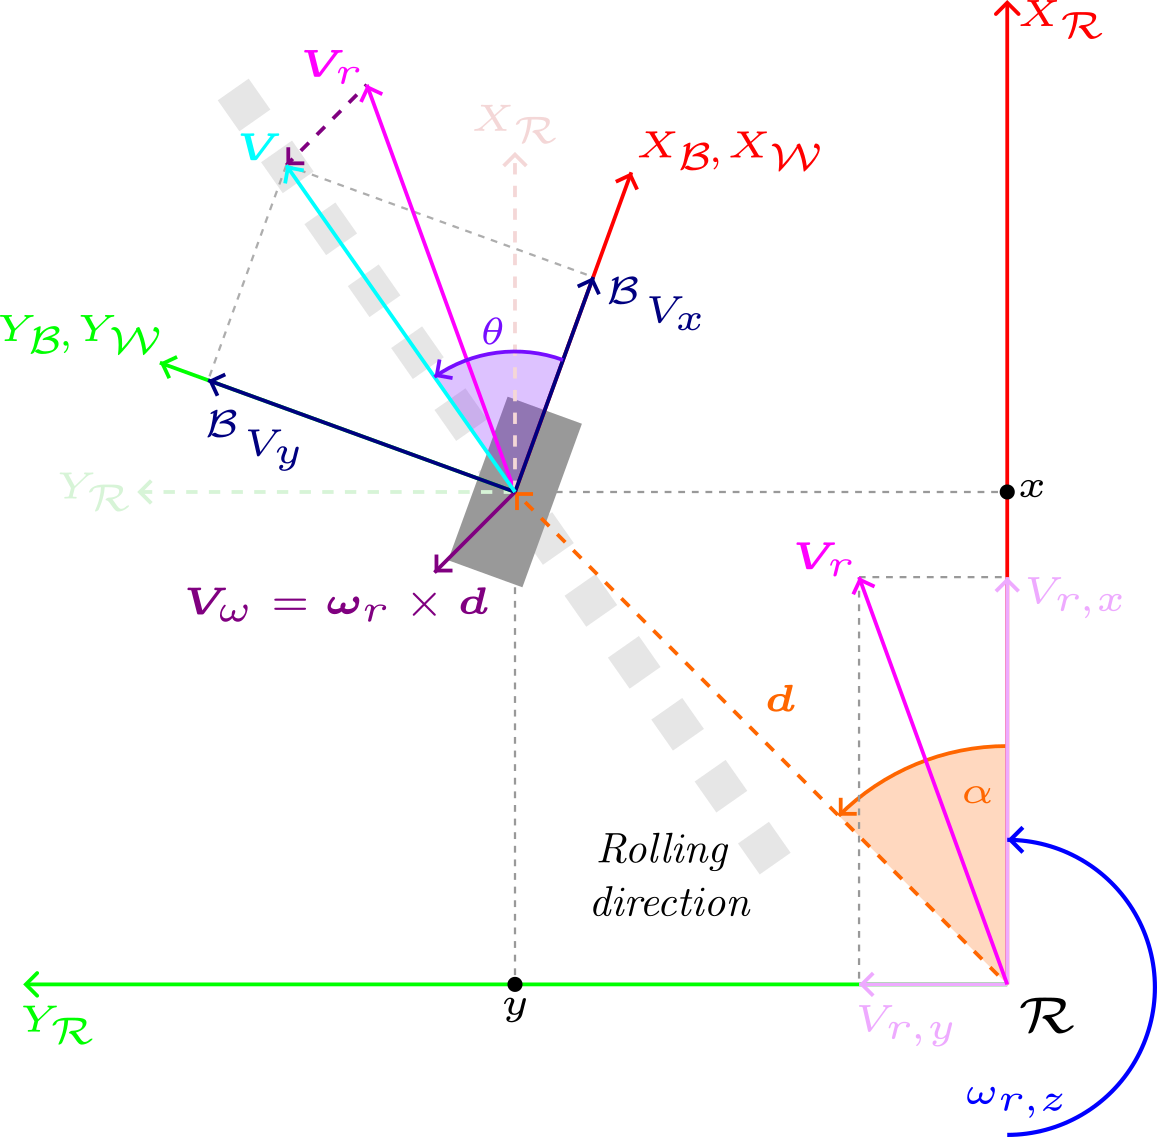
\includegraphics[width=1.0\linewidth]{images/wheel_vels.png}
    \caption{\(\vect{V}_r\) es el vector velocidad lineal del robot expresado en el SC \(\frameR\). \(\vect{V}_\omega\) es el vector velocidad tangencial de la rueda debido a la rotación del chasis. \(\vect{V}\) es el vector velocidad lineal de la rueda.}
    \label{fig:wheel-vels}
\end{figure}

La matriz que se conoce inicialmente es, \({}^\frameR R(\psi_i)_{\frameBi}\), que representa la orientación del SC \(\frameBi\) respecto del SC \(\frameR\).

\begin{equation}
    {}^\frameR  R(\psi_i)_{\frameBi} =
    \begin{bmatrix}
        \cos\psi_i & -\sin\psi_i           \\
        \sin\psi_i & \phantom{-}\cos\psi_i
    \end{bmatrix}
\end{equation}

con \(\psi_i = \phi_i - \frac{\pi}{2} = \alpha_i + \beta_i - \frac{\pi}{2}\).

Dado que las matrices de rotación son ortonormales, \(R^{-1} = R^{\trans}\), se puede obtener la matriz de rotación \({}^{\frameBi} R(\psi_i)_{\frameR}\) a partir de la matriz \({}^\frameR  R(\psi_i)_{\frameBi}\) fácilmente:

\begin{equation}
    {}^{\frameBi} R(\psi_i)_{\frameR} = \left({}^\frameR  R(\psi_i)_{\frameBi}\right)^{-1} = \left({}^\frameR  R(\psi_i)_{\frameBi}\right)^{\trans} =
    \begin{bmatrix}
        \phantom{-}\cos\psi_i & \sin\psi_i \\
        -\sin\psi_i           & \cos\psi_i
    \end{bmatrix}
    \label{eq:frameBi_R_frameR}
\end{equation}

A continuación se aplican las siguientes identidades trigonométricas en la expresión \ref{eq:frameBi_R_frameR}.

\[
    \begin{aligned}
        \cos\psi_i & = \cos\left(\phi_i - \frac{\pi}{2}\right) = \phantom{-}\sin\phi_i \\
        \sin\psi_i & = \sin\left(\phi_i - \frac{\pi}{2}\right) = -\cos\phi_i
    \end{aligned}
\]

\begin{equation}
    {}^{\frameBi}  R(\phi_i)_{\frameR} = \begin{bmatrix}
        \sin\phi_i & -\cos\phi_i           \\
        \cos\phi_i & \phantom{-}\sin\phi_i
    \end{bmatrix}
\end{equation}

Tras las simplificación, la expresión de la velocidad de la rueda \(i\) en el SC \(\frameBi\), \({}^{\frameBi} \vect{V}_i\), es:

\begin{equation}
    \begin{aligned}
        {}^{\frameBi} \vect{V}_i & = {}^{\frameBi} R(\phi_i)_{\frameR} \vect{V}_{i} = \begin{bmatrix}
                                                                                          \sin\phi_i & -\cos\phi_i           \\
                                                                                          \cos\phi_i & \phantom{-}\sin\phi_i
                                                                                      \end{bmatrix} \begin{bmatrix}
                                                                                                        1 & 0 & -d_{i} \sin\alpha_i           \\
                                                                                                        0 & 1 & \phantom{-}d_{i} \cos\alpha_i
                                                                                                    \end{bmatrix} \vect{V}_r =  \\
                                 & = \begin{bmatrix}
                                         \sin\phi_i & -\cos\phi_i           & -d_i(\phantom{-}\sin\alpha_i\sin\phi_i + \cos\alpha_i\cos\phi_i) \\
                                         \cos\phi_i & \phantom{-}\sin\phi_i & \phantom{-}d_i(-\sin\alpha_i\cos\phi_i + \cos\alpha_i\sin\phi_i)
                                     \end{bmatrix} \vect{V}_r
    \end{aligned}
    \label{eq:wheel-velocity-frameBi_expanded}
\end{equation}

A continuación se aplican las siguientes identidades trigonométricas a la expresión \ref{eq:wheel-velocity-frameBi_expanded} para simplificarla:

\[
    \begin{aligned}
        \phantom{-}\sin\alpha_i\sin\phi_i + \cos\alpha_i\cos\phi_i & = \cos(\phi_i - \alpha_i) = \cos((\alpha_i + \beta_i) - \alpha_i) = \cos\beta_i \\
        -\sin\alpha_i\cos\phi_i + \cos\alpha_i\sin\phi_i           & = \sin(\phi_i - \alpha_i) = \sin((\alpha_i + \beta_i) - \alpha_i) = \sin\beta_i
    \end{aligned}
\]

Tras la simplificación, la expresión de la velocidad de la rueda \(i\) en el SC \(\frameBi\), \({}^{\frameBi} \vect{V}_i\), es:

\begin{equation}
    ^{\frameBi}\vect{V}_{i} = \begin{bmatrix}
        \sin\phi_i & -\cos\phi_i           & -d_i\cos\beta_i           \\
        \cos\phi_i & \phantom{-}\sin\phi_i & \phantom{-}d_i\sin\beta_i
    \end{bmatrix} \vect{V}_r
    \label{eq:wheel-velocity-frameBi_final}
\end{equation}

Las restricciones físicas en el movimiento de la rueda \(i\), originadas por su contacto con el suelo, se describen de forma sencilla en su SC fijo, \(\frameWi\). Por tanto, para poder aplicar las restricciones físicas al movimiento de la rueda \(i\) de manera directa y sencilla, previamente hay que expresar su velocidad en el SC \(\frameWi\), \({}^{\frameWi} \vect{V}_i\).

\begin{equation}
    {}^{\frameWi} \vect{V}_i = \begin{bmatrix} v_{i\parallel} \\ v_{i\perp} \end{bmatrix}
\end{equation}

\begin{itemize}
    \item \(v_{i\parallel}\): componente de la velocidad de la rueda alineada con la dirección de rodadura, determinada por el eje \(\ejeXWi\).
    \item \(v_{i\perp}\): componente de la velocidad de la rueda alineada con la dirección de su eje de rotación, determinada por el eje \(\ejeYWi\) (dirección perpendicular a la dirección de rodadura).
\end{itemize}

\begin{equation}
    \begin{aligned}
        {}^{\frameWi} \vect{V}_i & = {}^{\frameWi} R(\theta_i)_{\frameBi} {}^{\frameBi} \vect{V}_i =                                     \\
                                 & = {}^{\frameWi} R(\theta_i)_{\frameBi} {}^{\frameBi} R(\phi_i)_{\frameR} \vect{V}_i =                 \\
                                 & = {}^{\frameWi} R(\theta_i)_{\frameBi} \begin{bmatrix}
                                                                              \sin\phi_i & -\cos\phi_i           & -d_i\cos\beta_i           \\
                                                                              \cos\phi_i & \phantom{-}\sin\phi_i & \phantom{-}d_i\sin\beta_i
                                                                          \end{bmatrix} \vect{V}_r
    \end{aligned}
    \label{eq:wheel-velocity-frameWi}
\end{equation}

La matriz \({}^{\frameWi} R(\theta_i)_{\frameBi}\) representa la orientación del SC \(\frameBi\) respecto del SC \(\frameWi\), y se usa para convertir vectores expresados en el SC \(\frameBi\) al SC \(\frameWi\).

De nuevo, dado que las matrices de rotación son ortonormales, se puede obtener la matriz de rotación \({}^{\frameWi} R(\theta_i)_{\frameBi}\) a partir de la matriz \({}^{\frameBi} R(\theta_i)_{\frameWi}\) fácilmente:

\begin{equation}
    \begin{aligned}
        {}^{\frameWi} R(\theta_i)_{\frameBi} & = \left({}^{\frameBi} R(\theta_i)_{\frameWi}\right)^{-1} = \left({}^{\frameBi} R(\theta_i)_{\frameWi}\right)^{\trans} = \begin{bmatrix}
                                                                                                                                                                           \cos\theta_i & -\sin\theta_i           \\
                                                                                                                                                                           \sin\theta_i & \phantom{-}\cos\theta_i
                                                                                                                                                                       \end{bmatrix}^{\trans} = \\
                                             & = \begin{bmatrix}
                                                     \phantom{-}\cos\theta_i & \sin\theta_i \\
                                                     -\sin\theta_i           & \cos\theta_i
                                                 \end{bmatrix}
    \end{aligned}
\end{equation}

\begin{equation}
    \begin{aligned}
        {}^{\frameWi} \vect{V}_i & = \begin{bmatrix}
                                         \phantom{-}\cos\theta_i & \sin\theta_i \\
                                         -\sin\theta_i           & \cos\theta_i
                                     \end{bmatrix} {}^{\frameBi} \vect{V}_i =                                                                                                \\
                                 & = \begin{bmatrix}
                                         \phantom{-}\cos\theta_i & \sin\theta_i \\
                                         -\sin\theta_i           & \cos\theta_i
                                     \end{bmatrix} \begin{bmatrix}
                                                       \sin\phi_i & -\cos\phi_i           \\
                                                       \cos\phi_i & \phantom{-}\sin\phi_i
                                                   \end{bmatrix} \vect{V}_i =                                                                                        \\
                                 & = \begin{bmatrix}
                                         \phantom{-}\cos\theta_i & \sin\theta_i \\
                                         -\sin\theta_i           & \cos\theta_i
                                     \end{bmatrix} \begin{bmatrix}
                                                       \sin\phi_i & -\cos\phi_i           \\
                                                       \cos\phi_i & \phantom{-}\sin\phi_i
                                                   \end{bmatrix}\begin{bmatrix}
                                                                    1 & 0 & -d_{i} \sin\alpha_i           \\
                                                                    0 & 1 & \phantom{-}d_{i} \cos\alpha_i
                                                                \end{bmatrix} \vect{V}_r =                                                                        \\
                                 & = \begin{bmatrix}
                                         \phantom{-}\cos\theta_i & \sin\theta_i \\
                                         -\sin\theta_i           & \cos\theta_i
                                     \end{bmatrix} \begin{bmatrix}
                                                       \sin\phi_i & -\cos\phi_i           & -d_i\cos\beta_i           \\
                                                       \cos\phi_i & \phantom{-}\sin\phi_i & \phantom{-}d_i\sin\beta_i
                                                   \end{bmatrix} \vect{V}_r =                                                            \\
                                 & = \begin{bmatrix}
                                         \sin\left(\phi_i + \theta_i \right) & -\cos\left(\phi_i + \theta_i\right)           & -d_i\cos\left(\beta_i + \theta_i\right)           \\
                                         \cos\left(\phi_i + \theta_i\right)  & \phantom{-}\sin\left(\phi_i + \theta_i\right) & \phantom{-}d_i\sin\left(\beta_i + \theta_i\right)
                                     \end{bmatrix} \vect{V}_r
    \end{aligned}
    \label{eq:wheel-velocity-frameWi_final}
\end{equation}

En la expresión \ref{eq:wheel-velocity-frameWi_final} se han aplicado las siguientes identidades trigonométricas:

\[
    \begin{aligned}
        \cos\theta_i\sin\phi_i + \sin\theta_i\cos\phi_i & = \sin\left(\theta_i + \phi_i\right) \\
        \cos\theta_i\cos\phi_i - \sin\theta_i\sin\phi_i & = \cos\left(\theta_i + \phi_i\right)
    \end{aligned}
\]

Para cada rueda \(i\) se obtiene un sistema de 2 ecuaciones lineales con 3 incógnitas: \(V_{r,x}\), \(V_{r,y}\) y \(\omega_{r,z}\).

Para \(N\) ruedas se obtienen \(2N\) ecuaciones lineales y 3 incógnitas. Por tanto, para \(N \ge 2\) el sistema es sobredeterminado (\(2N > 3\)).

Dependiendo de si las ruedas usadas en una plataforma son convencionales no orientables, convencionales orientables, mecanum u omnidireccionales, se aplicarán diferentes restricciones físicas a las componentes \(v_{i\parallel}\) y \(v_{i\perp}\), lo que dará lugar a expresiones específicas que resuelven la cinemática directa e inversa para la plataforma considerada. Ver figura \ref{fig:wheel-vels-2}.

\begin{figure}[H]
    \centering
    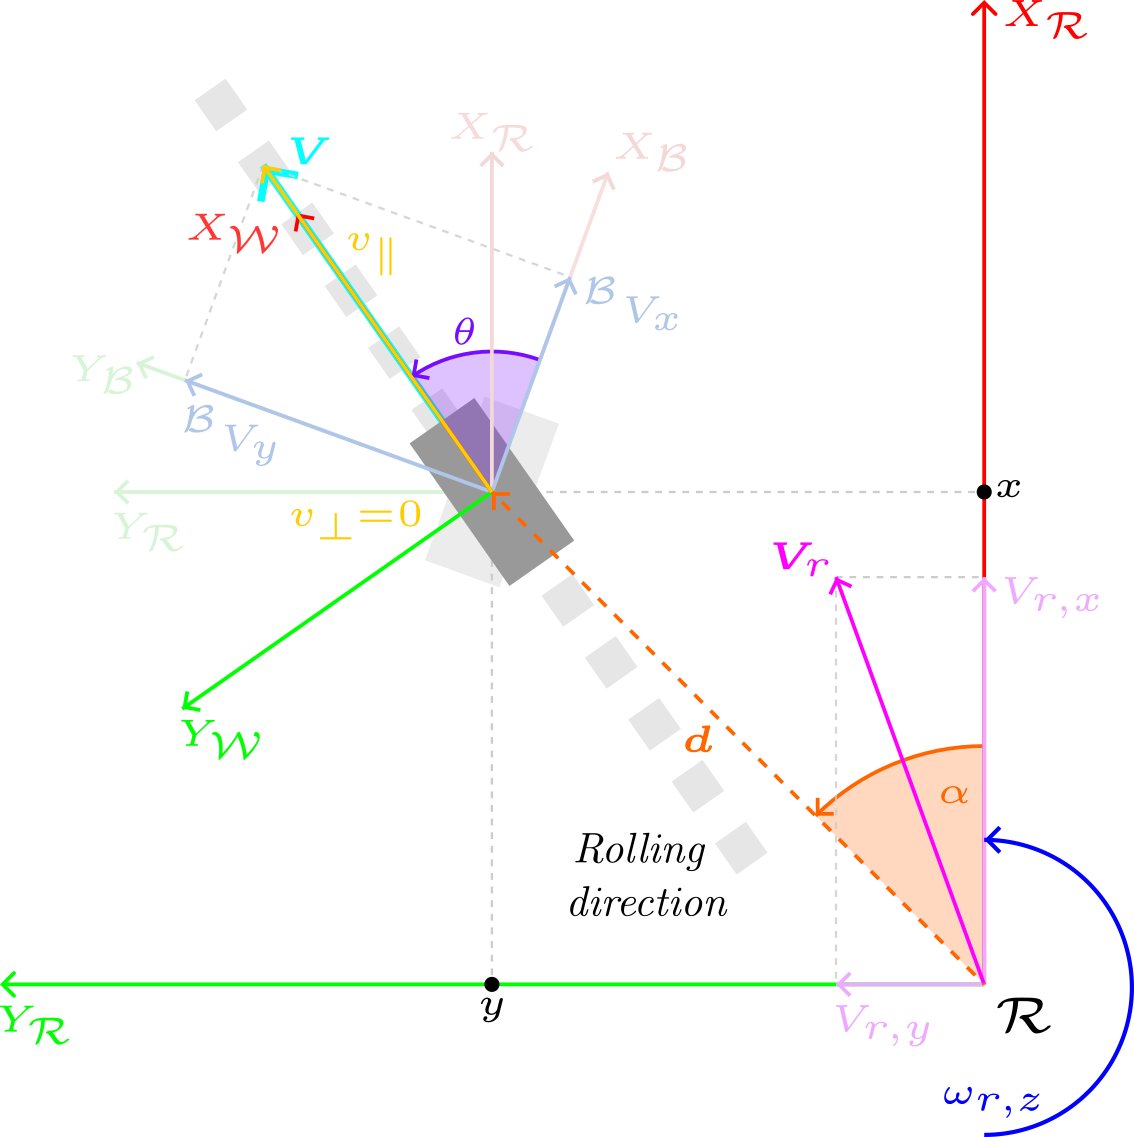
\includegraphics[width=1.0\linewidth]{images/wheel_vels_2.png}
    \caption{Relación entre el vector velocidad de la rueda en el SC \(\frameB\), \({}^\frameB \vect{V}\) y en el SC \(\frameW\), \({}^\frameW \vect{V}\) para una rueda convencional orientable.}
    \label{fig:wheel-vels-2}
\end{figure}

\section{Consideraciones generales sobre cinemática directa e inversa}
\label{sec:general-considerations}

En general, la cinemática directa e inversa de un robot terrestre queda definido mediante una expresión matricial de la forma:

\begin{equation}
    A\mathbf{x} = \mathbf{b}
\end{equation}

donde:

\[
    A \in \mathbb{R}^{2N \times 3}, \quad \mathbf{x} \in \mathbb{R}^3, \quad \mathbf{b} \in \mathbb{R}^{2N}
\]

Para acortar la notación, se usan los siguientes símbolos:

\[
    \begin{aligned}
        \lambda_i & = \phi_i + \theta_i  \\
        \gamma_i  & = \beta_i + \theta_i
    \end{aligned}
\]

\[
    A = \begin{bmatrix}
        \sin\left(\lambda_0\right)     & -\cos\left(\lambda_0\right)               & -d_0\cos\left(\gamma_0\right)                   \\
        \cos\left(\lambda_0\right)     & \phantom{-}\sin\left(\lambda_0\right)     & \phantom{-}d_0\sin\left(\gamma_0\right)         \\
        \vdots                         & \vdots                                    & \vdots                                          \\
        \sin\left(\lambda_{N-1}\right) & -\cos\left(\lambda_{N-1}\right)           & -d_{N-1}\cos\left(\gamma_{N-1}\right)           \\
        \cos\left(\lambda_{N-1}\right) & \phantom{-}\sin\left(\lambda_{N-1}\right) & \phantom{-}d_{N-1}\sin\left(\gamma_{N-1}\right)
    \end{bmatrix}
\]

\[
    \mathbf{x} =
    \begin{bmatrix}
        V_{r,x} \\
        V_{r,y} \\
        \omega_{r,z}
    \end{bmatrix}, \quad \mathbf{b} = \begin{bmatrix}
        v_{0\parallel}   \\
        v_{0\perp}       \\
        \vdots           \\
        v_{N-1\parallel} \\
        v_{N-1\perp}
    \end{bmatrix}
\]

Dado que para cualquier robot con \(N \ge 2\) ruedas se obtienen \(2N\) ecuaciones y únicamente 3 incógnitas, nos encontramos ante un sistema lineal sobredeterminado.

En un escenario ideal puramente matemático, bastaría con tomar cualquier subconjunto de 3 ecuaciones linealmente independientes para resolver el sistema y hallar la velocidad del chasis, \(\mathbf{x}\). Sin embargo, en la implementación real de un robot terrestre, las ecuaciones nunca encajan de forma perfecta debido a imperfecciones como:

\begin{itemize}
    \item Ruido y cuantización en la lectura de los sensores (encoders).
    \item Pequeños deslizamientos de las ruedas sobre el terreno.
    \item Ligeras desviaciones en la calibración geométrica de la base.
\end{itemize}

Por tanto, el sistema no se resuelve buscando una solución algebraica exacta, sino buscando la estimación \(\hat{\mathbf{x}}\) que minimice el error cuadrático global de todas las ruedas simultáneamente:

\begin{equation}
    \hat{\mathbf{x}} = \arg\min_{\mathbf{x}} \|A\mathbf{x} - \mathbf{b}\|^2
\end{equation}

La solución a este problema de mínimos cuadrados viene dada por la expresión conocida como Ecuaciones Normales, que se obtiene de un proceso de búsqueda del mínimo de la función de error (derivando e igualando a cero):

\begin{equation}
    A^{\trans} A \mathbf{x} = A^{\trans} \mathbf{b}
\end{equation}

Por tanto, la solución óptima se obtiene mediante:

\begin{equation}
    \hat{\mathbf{x}} = (A^{\trans}A)^{-1}A^{\trans}\mathbf{b} = A^+\mathbf{b}
\end{equation}

donde \(A^+\) se denomina la pseudoinversa de Moore-Penrose de la matriz \(A\).

Desde el punto de vista del cálculo numérico computacional, invertir directamente la matriz \((A^{\trans}A)\) puede ser inestable si la matriz original \(A\) está mal condicionada. Una matriz se considera mal condicionada cuando pequeñas variaciones o ruidos en los datos de entrada (el vector \(\mathbf{b}\)) se amplifican drásticamente, provocando cálculos erráticos en la solución resultante \(\hat{\mathbf{x}}\).

El mal comportamiento numérico que puede surgir al usar la fórmula de ecuaciones normales se debe a que el término \((A^{\trans}A)^{-1}\allowbreak A^{\trans}\) eleva al cuadrado los valores singulares de \(A\). Si \(A\) tiene un valor singular pequeño, cercano a cero, al elevarlo al cuadrado se vuelve aún más pequeño. Al intentar invertir ese valor, el ordenador divide por un número casi cero, lo que hace que los resultados se disparen a infinito y se pierda toda la precisión en la solución.

Aunque no es estrictamente necesario para el desarrollo de la cinemática, por completitud se indica que para averiguar la robustez geométrica de la matriz \(A\) se utiliza el cociente entre su valor singular máximo y mínimo (\(\kappa = \frac{\sigma_{\max}}{\sigma_{\min}}\)), denominado \textbf{número de condición}, \(\kappa(A)\). A modo de referencia:

\begin{itemize}
    \item \(\kappa = 1\): \(A\) es la matriz perfecta (ejemplo: la matriz Identidad o una matriz de rotación pura). No hay pérdida de precisión.
    \item \(1 < \kappa < 10^2\): \(A\) está bien condicionada. El sistema es robusto; los errores de los sensores no se amplificarán significativamente.
    \item \(10^3 < \kappa < 10^6\): \(A\) está medianamente mal condicionada. Se debe tener precaución, ya que los métodos simples como invertir \((A^{\trans}A)\) pueden empezar a dar resultados imprecisos.
    \item \(\kappa \approx 10^{12} \text{ a } 10^{15}\): \(A\) está mal condicionada. La matriz es casi singular (sus filas/columnas son casi dependientes).
    \item \(\kappa > 10^{16}\): \(A\) es singular e inutilizable. Para una computadora que trabaja con precisión doble (64 bits), esto significa que la matriz no se puede invertir con fiabilidad.
\end{itemize}

Para evitar estos problemas de estabilidad numérica que podrían llegar a darse, en la práctica se obtiene la pseudoinversa \(A^+\) aplicando la Descomposición en Valores Singulares (SVD) a la matriz original \(A\). La SVD es el método numérico más robusto y seguro, ya que evita por completo el producto \((A^{\trans}A)\) y es capaz de manejar matrices casi-singulares (situaciones donde las ecuaciones geométricas del robot son tan parecidas o redundantes que el sistema está al borde de no poder invertirse) sin que los cálculos resultantes se disparen a infinito. Este método funciona incluso si la matriz \(A\) no tiene rango completo (si algunas de las ecuaciones son directamente contradictorias).

Sin embargo, es fundamental hacer una distinción crítica entre la robustez matemática del software y la viabilidad física del robot. Si al evaluar la matriz geométrica constante \(A\) durante la fase de diseño se obtiene un número de condición elevado (por ejemplo, \(\kappa > 10^3\), y críticamente si \(\kappa > 10^6\)), \textbf{sucederá que, aunque el algoritmo SVD evite el colapso del programa devolviendo una solución matemática estable (al truncar los valores casi nulos), en realidad se estará enmascarando un defecto grave en el diseño mecánico.} Físicamente, esto significa que la disposición constructiva de las ruedas (sus distancias \(d_i\) o ángulos de montaje \(\alpha_i, \beta_i\)) genera una cinemática degenerada, donde el chasis pierde capacidad para moverse de forma independiente en todos sus grados de libertad, o donde las direcciones de rodadura entran en conflicto directo. En este escenario, aunque el software entregue un resultado numérico aparentemente válido, el robot físico sufrirá derivas incontrolables, estrés mecánico y movimientos erráticos ante el más mínimo ruido en los encoders. Por tanto, la SVD no debe usarse como un pretexto para ignorar una mala geometría; si el número de condición inicial es excesivamente alto, la solución ineludible pasa por replantear la ubicación y orientación base de las ruedas en el diseño CAD hasta lograr un sistema bien condicionado (idealmente \(\kappa \le 100\)).

La SVD descompone la matriz en \(A = U \Sigma V^{\trans}\), permitiendo construir la pseudoinversa directamente como \(A^+ = V \Sigma^+ U^{\trans}\).

\textbf{Demostración:}

Si \(A = U \Sigma V^{\trans}\), se aplica la propiedad de la transpuesta para un producto de matrices: \((X Y Z)^{\trans} = Z^{\trans} Y^{\trans} X^{\trans}\) (el orden se invierte).

\begin{equation}
    A^{\trans} = (V^{\trans})^{\trans} \Sigma^{\trans} U^{\trans}
\end{equation}

Transponer dos veces devuelve la matriz original (\((V^{\trans})^{\trans} = V\)), y como \(\Sigma\) es una matriz diagonal que no cambia al transponerse (\(\Sigma^{\trans} = \Sigma\))\footnote{Para que la igualdad \(\Sigma^{\trans} = \Sigma\) sea estrictamente cierta, \(\Sigma\) tiene que ser una matriz cuadrada. En sistemas sobredeterminados, donde \(A\) es una matriz rectangular de \(M \times N\), la matriz \(\Sigma\) original es rectangular de \(M \times N\) y \(\Sigma^{\trans}\) sería de \(N \times M\), por lo que no se cumpliría la igualdad. Sin embargo, en la práctica, para resolver estos sistemas se suele emplear la SVD Reducida (o \textit{Thin SVD}), que recorta las filas de ceros de la matriz \(\Sigma\), convirtiéndola en una matriz cuadrada de tamaño \(N \times N\). De esta forma, sí se cumple que \(\Sigma^{\trans} = \Sigma\) en la SVD Reducida, lo que permite desarrollar la fórmula \(A^+ = V \Sigma^+ U^{\trans}\) sin conflictos dimensionales. En la librería Eigen de C++, la combinación de opciones \texttt{ComputeThinU | ComputeThinV} realiza exactamente este cálculo.}, se obtiene:

\begin{equation}
    A^{\trans} = V \Sigma U^{\trans}
\end{equation}

Sustituyendo en el producto \(A^{\trans} A\):

\begin{equation}
    A^{\trans} A = (V \Sigma U^{\trans}) (U \Sigma V^{\trans})
\end{equation}

Por la propiedad asociativa de las matrices, se pueden omitir los paréntesis internos:

\begin{equation}
    A^{\trans} A = V \Sigma (U^{\trans} U) \Sigma V^{\trans}
\end{equation}

La matriz \(U\) es ortogonal, lo que significa que su transpuesta multiplicada por sí misma da como resultado la matriz Identidad (\(U^{\trans} U = I\)):

\begin{equation}
    A^{\trans} A = V \Sigma I \Sigma V^{\trans}
\end{equation}

Multiplicar por la matriz Identidad no altera el resultado, y \(\Sigma\) multiplicada por sí misma es \(\Sigma^2\) (que equivale a elevar al cuadrado los valores de su diagonal):

\begin{equation}
    A^{\trans} A = V \Sigma^2 V^{\trans}
\end{equation}

A continuación, se aplica la inversa a toda la expresión utilizando la propiedad de la inversa para un producto: \((X Y Z)^{-1} = Z^{-1} Y^{-1} X^{-1}\).

\begin{equation}
    (A^{\trans} A)^{-1} = (V^{\trans})^{-1} (\Sigma^2)^{-1} V^{-1}
\end{equation}

Como \(V\) también es una matriz ortogonal, su inversa es igual a su transpuesta, \(V^{-1} = V^{\trans}\), y, por tanto, \((V^{\trans})^{-1} = V\). La inversa de una matriz diagonal \(\Sigma^2\) se denota simplemente como \(\Sigma^{-2}\) (que consiste en invertir los valores elevados al cuadrado de su diagonal). Sustituyendo estas propiedades, se obtiene:

\begin{equation}
    (A^{\trans} A)^{-1} = V \Sigma^{-2} V^{\trans}
\end{equation}

Se multiplica ahora por \(A^{\trans}\) por la derecha para completar la expresión de las Ecuaciones Normales:

\begin{equation}
    (A^{\trans} A)^{-1} A^{\trans} = (V \Sigma^{-2} V^{\trans}) (V \Sigma U^{\trans})
\end{equation}

Se quitan de nuevo los paréntesis internos por la propiedad asociativa:

\begin{equation}
    (A^{\trans} A)^{-1} A^{\trans} = V \Sigma^{-2} (V^{\trans} V) \Sigma U^{\trans}
\end{equation}

Nuevamente, dado que \(V\) es ortogonal, \(V^{\trans} V = I\). El término central desaparece:

\begin{equation}
    (A^{\trans} A)^{-1} A^{\trans} = V \Sigma^{-2} \Sigma U^{\trans}
\end{equation}

En este punto se tiene \(\Sigma^{-2}\) multiplicado por \(\Sigma\). Debido a que ambas son matrices diagonales, la operación equivale a multiplicar cada elemento de la diagonal de \(\Sigma^{-2}\) por el correspondiente elemento de la diagonal de \(\Sigma\). De modo que cada elemento de la diagonal resultante es el valor original de \(\Sigma\) elevado a \(-2 + 1 = -1\) (es decir, el inverso de los valores originales de \(\Sigma\)). A esta matriz diagonal resultante se le denota como \(\Sigma^+\):

\begin{itemize}
    \item Si \(A\) \textbf{no} tiene rango completo, \(\Sigma^+\) se define como la matriz diagonal que contiene el inverso de los valores singulares no nulos de \(A\), y ceros en las posiciones correspondientes a los valores singulares nulos.
    \item Si \(A\) \textbf{tiene} rango completo, entonces \(\Sigma^+\) es en realidad \(\Sigma^{-1}\) (una inversa propiamente dicha), que es la matriz diagonal que contiene el inverso de todos los valores singulares de \(A\).
\end{itemize}

Finalmente, sustituyendo \(\Sigma^+\), se llega a la expresión:

\begin{equation}
    (A^{\trans} A)^{-1} A^{\trans} = V \Sigma^+ U^{\trans}
\end{equation}

Como se comentó anteriormente, el problema computacional surge cuando el ordenador evalúa la expresión \((A^{\trans} A)^{-1}\) directamente, ya que debe elevar al cuadrado valores singulares que podrían ser muy cercanos a cero. Al intentar invertir esos valores casi nulos elevados al cuadrado, se producen desbordamientos numéricos. Usando la fórmula final directa \(V \Sigma^+ U^{\trans}\) proporcionada por la SVD, el algoritmo únicamente invierte los valores originales (\(\Sigma^+\)), manteniendo el sistema estable en todo momento.

\section{Cinemática de un robot con base three swerve drive}

La base con tres ruedas activas orientables (three swerve drive) es un sistema de locomoción omnidireccional. Permite que un robot terrestre se mueva en cualquier dirección sin tener que cambiar antes la orientación del chasis. Cada rueda se orienta de forma independiente, por lo que el robot gana maniobrabilidad y flexibilidad.

\begin{figure}[H]
    \centering
    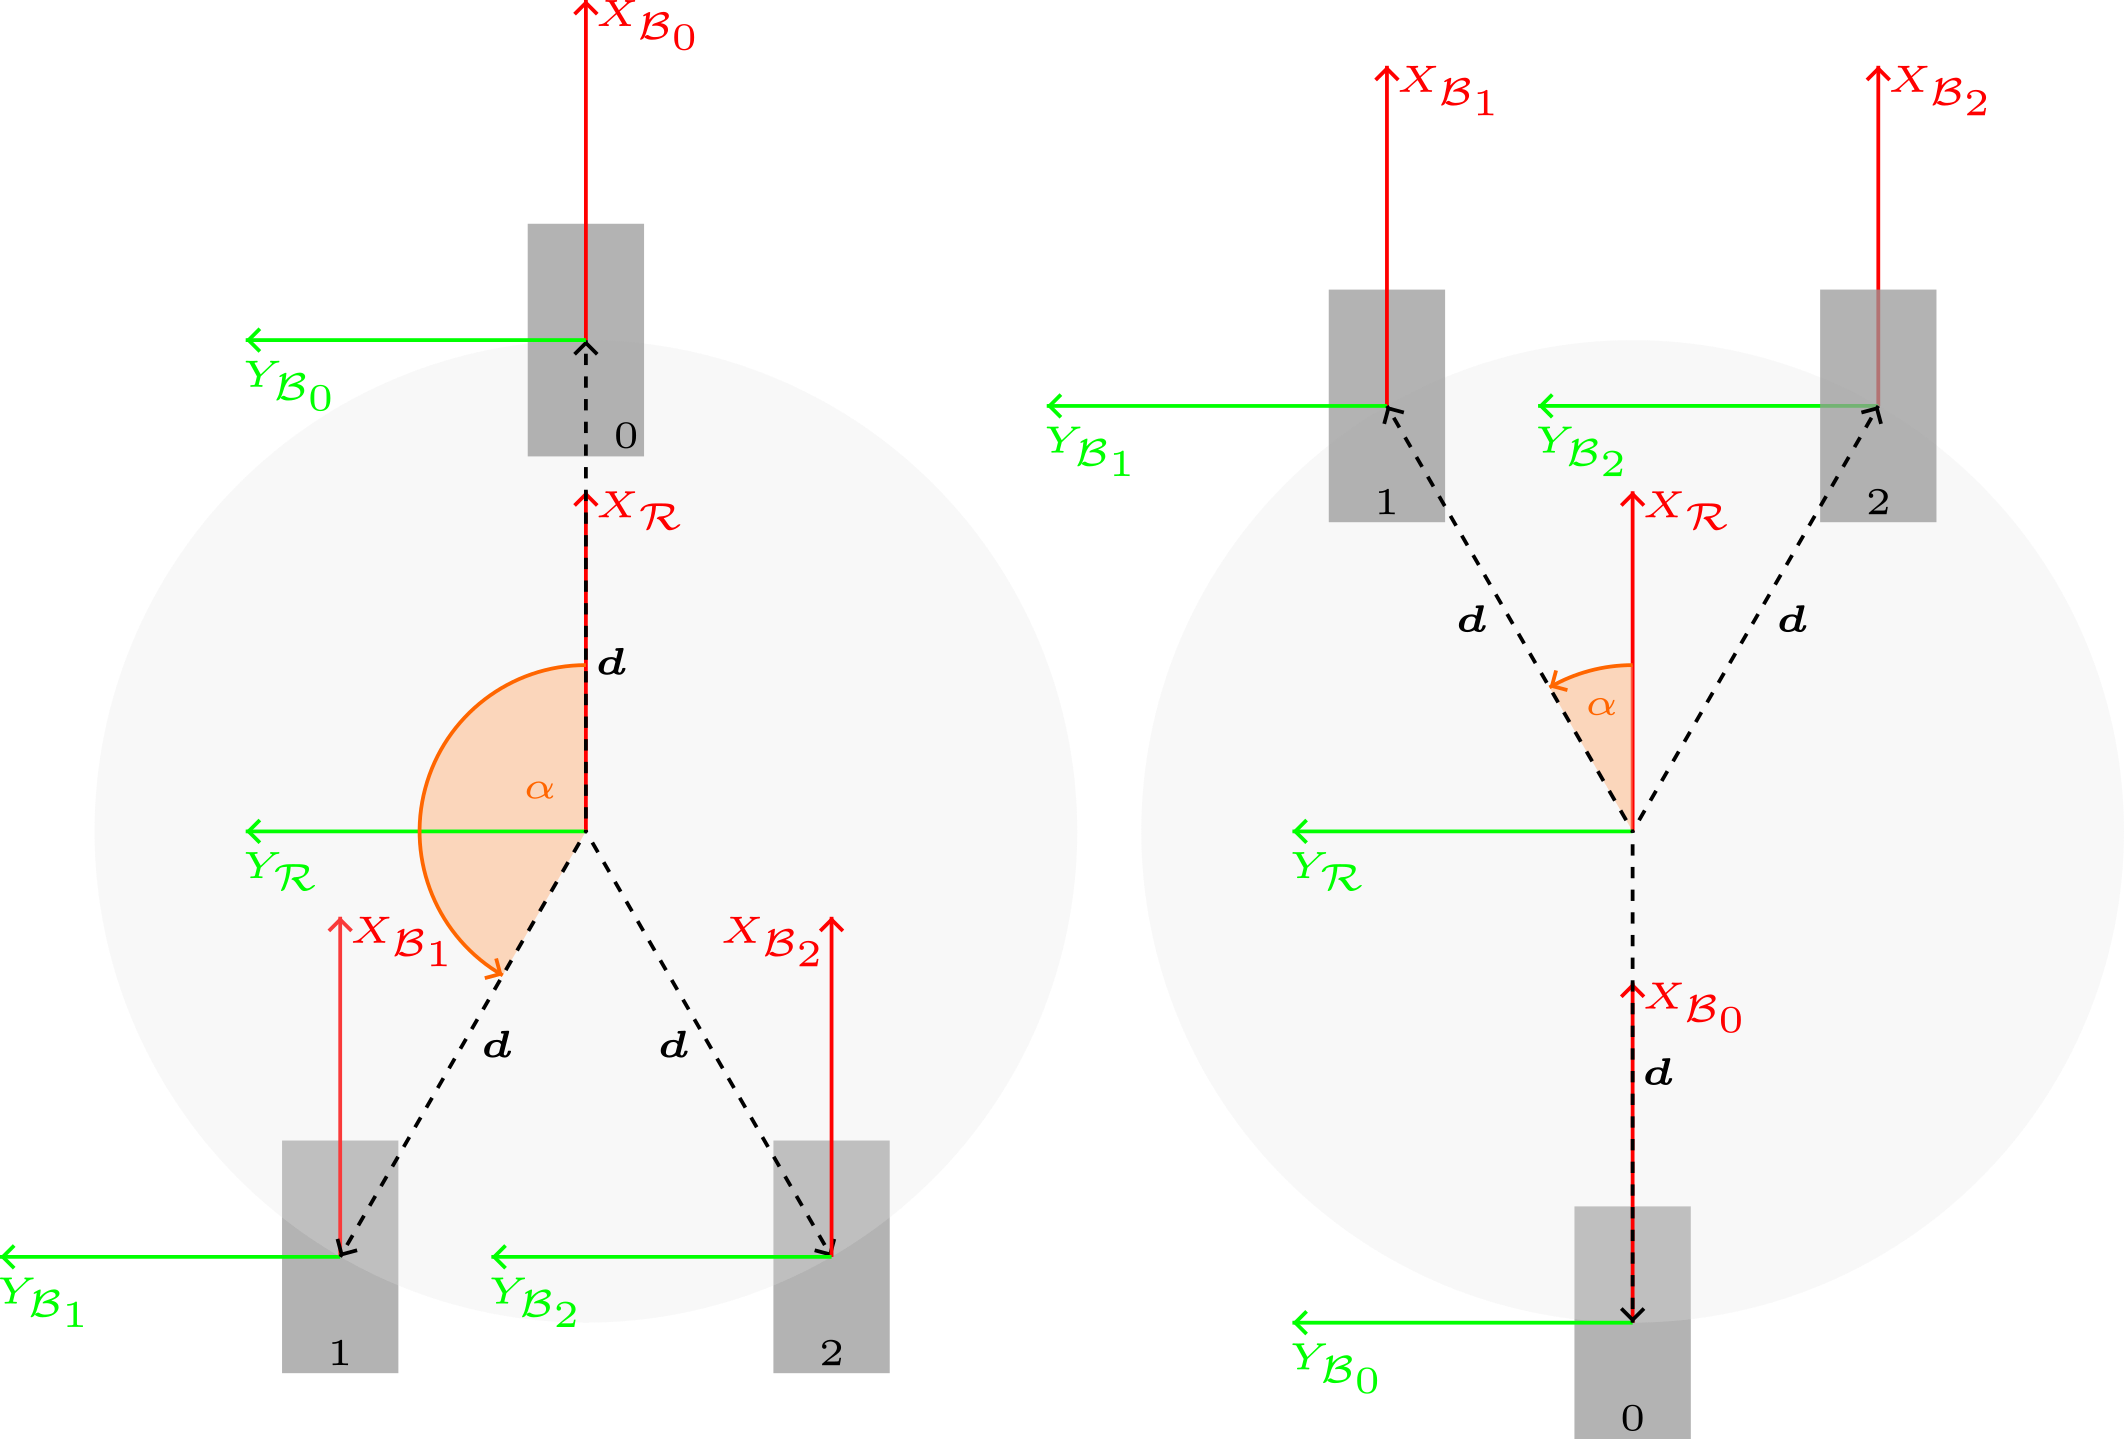
\includegraphics[width=1.0\linewidth]{images/three_swerve_drive_configuration.png}
    \caption{Configuraciones comunes de las ruedas en un sistema three swerve drive (izquierda: configuración Y-invertida, derecha: configuración Y)}
    \label{fig2:three-swerve-drive-configuration}
\end{figure}

Todas las ruedas tienen el mismo radio \(r\) y están situadas a la misma distancia \(d\) del centro de la base.

Además, en este caso particular se impone:

\[
    \begin{aligned}
        \psi_i = \phi_i - \frac{\pi}{2} = 0 \quad          & \Longrightarrow \quad \phi_i = \frac{\pi}{2}             \\
        \phi_i = \alpha_i + \beta_i = \frac{\pi}{2}, \quad & \Longrightarrow \quad \beta_i = \frac{\pi}{2} - \alpha_i
    \end{aligned}
\]

y por tanto:

\[
    {}^{\frameBi} R\left(\phi_i = \frac{\pi}{2}\right)_{\frameR} = \begin{bmatrix}
        \sin\frac{\pi}{2} & -\cos\frac{\pi}{2}           \\
        \cos\frac{\pi}{2} & \phantom{-}\sin\frac{\pi}{2}
    \end{bmatrix} = \begin{bmatrix}
        1 & 0 \\
        0 & 1
    \end{bmatrix}
\]

Para la configuración Y-invertida:

\begin{itemize}
    \item \(\alpha \in \left[\frac{\pi}{2}, \pi\right)\) y \(d > 0\)
    \item Rueda frontal \((i = 0)\):
          \[
              \begin{aligned}
                  \alpha_0   & = 0                                                              \\
                  \vect{d}_0 & = (d\cos\alpha_0,\ d\sin\alpha_0) = (d\cos 0,\ d\sin 0) = (d, 0) \\
                  \beta_0    & =\frac{\pi}{2} - \alpha_0 = \frac{\pi}{2} - 0 = \frac{\pi}{2}
              \end{aligned}
          \]
    \item Rueda izquierda \((i = 1)\):
          \[
              \begin{aligned}
                  \alpha_1   & = \alpha                                                      \\
                  \vect{d}_1 & = (d\cos\alpha_1, d\sin\alpha_1) = (d\cos\alpha, d\sin\alpha) \\
                  \beta_1    & = \frac{\pi}{2} - \alpha_1 = \frac{\pi}{2} - \alpha
              \end{aligned}
          \]
    \item Rueda derecha \((i = 2)\):
          \[
              \begin{aligned}
                  \alpha_2   & = -\alpha                                                                                         \\
                  \vect{d}_2 & = (d\cos\alpha_2, d\sin\alpha_2) = (d\cos(-\alpha), d\sin(-\alpha)) = (d\cos\alpha, -d\sin\alpha) \\
                  \beta_2    & = \frac{\pi}{2} - \alpha_2 = \frac{\pi}{2} - (-\alpha) = \frac{\pi}{2} + \alpha
              \end{aligned}
          \]
\end{itemize}

A continuación se presenta la matriz \(A\) para la configuración Y-invertida:

\begin{equation}
    \begin{aligned}
        A & = \begin{bmatrix}
                  \sin\phi_0 & -\cos\phi_0           & -d_0\cos\beta_0           \\
                  \cos\phi_0 & \phantom{-}\sin\phi_0 & \phantom{-}d_0\sin\beta_0 \\
                  \sin\phi_1 & -\cos\phi_1           & -d_1\cos\beta_1           \\
                  \cos\phi_1 & \phantom{-}\sin\phi_1 & \phantom{-}d_1\sin\beta_1 \\
                  \sin\phi_2 & -\cos\phi_2           & -d_2\cos\beta_2           \\
                  \cos\phi_2 & \phantom{-}\sin\phi_2 & \phantom{-}d_2\sin\beta_2
              \end{bmatrix} = \begin{bmatrix}
                                  1 & 0 & -d\cos\left(\frac{\pi}{2}- \alpha_0\right)            \\
                                  0 & 1 & \phantom{-}d\sin\left(\frac{\pi}{2} - \alpha_0\right) \\
                                  1 & 0 & -d\cos\left(\frac{\pi}{2}-\alpha_1\right)             \\
                                  0 & 1 & \phantom{-}d\sin\left(\frac{\pi}{2}-\alpha_1\right)   \\
                                  1 & 0 & -d\cos\left(\frac{\pi}{2}-\alpha_2\right)             \\
                                  0 & 1 & \phantom{-}d\sin\left(\frac{\pi}{2}-\alpha_2\right)
                              \end{bmatrix}  = \\
          & = \begin{bmatrix}
                  1 & 0 & -d\sin\alpha_0           \\
                  0 & 1 & \phantom{-}d\cos\alpha_0 \\
                  1 & 0 & -d\sin\alpha_1           \\
                  0 & 1 & \phantom{-}d\cos\alpha_1 \\
                  1 & 0 & -d\sin\alpha_2           \\
                  0 & 1 & \phantom{-}d\cos\alpha_2
              \end{bmatrix} = \begin{bmatrix}
                                  1 & 0 & -y_0           \\
                                  0 & 1 & \phantom{-}x_0 \\
                                  1 & 0 & -y_1           \\
                                  0 & 1 & \phantom{-}x_1 \\
                                  1 & 0 & -y_2           \\
                                  0 & 1 & \phantom{-}x_2
                              \end{bmatrix}
    \end{aligned}
\end{equation}

Para la configuración Y:

\begin{itemize}
    \item \(\alpha \in \left(0, \frac{\pi}{2}\right]\) y \(d > 0\)
    \item Rueda trasera \((i = 0)\):
          \[
              \begin{aligned}
                  \alpha_0   & = \pi                                                             \\
                  \vect{d}_0 & = (d\cos\alpha_0, d\sin\alpha_0) = (d\cos\pi, d\sin\pi) = (-d, 0) \\
                  \beta_0    & = \frac{\pi}{2} - \alpha_0 = \frac{\pi}{2} - \pi = -\frac{\pi}{2}
              \end{aligned}
          \]
    \item Rueda izquierda \((i = 1)\):
          \[
              \begin{aligned}
                  \alpha_1   & = \alpha                                                      \\
                  \vect{d}_1 & = (d\cos\alpha_1, d\sin\alpha_1) = (d\cos\alpha, d\sin\alpha) \\
                  \beta_1    & = \frac{\pi}{2} - \alpha_1 = \frac{\pi}{2} - \alpha
              \end{aligned}
          \]
    \item Rueda derecha \((i = 2)\):
          \[
              \begin{aligned}
                  \alpha_2   & = -\alpha                                                                                         \\
                  \vect{d}_2 & = (d\cos\alpha_2, d\sin\alpha_2) = (d\cos(-\alpha), d\sin(-\alpha)) = (d\cos\alpha, -d\sin\alpha) \\
                  \beta_2    & = \frac{\pi}{2} - \alpha_2 = \frac{\pi}{2} - (-\alpha) = \frac{\pi}{2} + \alpha
              \end{aligned}
          \]
\end{itemize}

A continuación se presenta la matriz \(A\) para la configuración Y:

\begin{equation}
    \begin{aligned}
        A & = \begin{bmatrix}
                  \sin\phi_0 & -\cos\phi_0           & -d_0\cos\beta_0           \\
                  \cos\phi_0 & \phantom{-}\sin\phi_0 & \phantom{-}d_0\sin\beta_0 \\
                  \sin\phi_1 & -\cos\phi_1           & -d_1\cos\beta_1           \\
                  \cos\phi_1 & \phantom{-}\sin\phi_1 & \phantom{-}d_1\sin\beta_1 \\
                  \sin\phi_2 & -\cos\phi_2           & -d_2\cos\beta_2           \\
                  \cos\phi_2 & \phantom{-}\sin\phi_2 & \phantom{-}d_2\sin\beta_2
              \end{bmatrix} = \begin{bmatrix}
                                  1 & 0 & -d\cos\left(\frac{\pi}{2} - \alpha_0\right)           \\
                                  0 & 1 & \phantom{-}d\sin\left(\frac{\pi}{2} - \alpha_0\right) \\
                                  1 & 0 & -d\cos\left(\frac{\pi}{2} - \alpha_1\right)           \\
                                  0 & 1 & \phantom{-}d\sin\left(\frac{\pi}{2} - \alpha_1\right) \\
                                  1 & 0 & -d\cos\left(\frac{\pi}{2} - \alpha_2\right)           \\
                                  0 & 1 & \phantom{-}d\sin\left(\frac{\pi}{2} - \alpha_2\right)
                              \end{bmatrix}  = \\
          & = \begin{bmatrix}
                  1 & 0 & -d\sin\alpha_0           \\
                  0 & 1 & \phantom{-}d\cos\alpha_0 \\
                  1 & 0 & -d\sin\alpha_1           \\
                  0 & 1 & \phantom{-}d\cos\alpha_1 \\
                  1 & 0 & -d\sin\alpha_2           \\
                  0 & 1 & \phantom{-}d\cos\alpha_2
              \end{bmatrix} = \begin{bmatrix}
                                  1 & 0 & -y_0           \\
                                  0 & 1 & \phantom{-}x_0 \\
                                  1 & 0 & -y_1           \\
                                  0 & 1 & \phantom{-}x_1 \\
                                  1 & 0 & -y_2           \\
                                  0 & 1 & \phantom{-}x_2
                              \end{bmatrix}
    \end{aligned}
\end{equation}

Por lo tanto, se demuestra que ambas configuraciones, Y-invertida y Y, comparten la misma matriz \(A\), lo que implica que su cinemática directa e inversa es idéntica. La única diferencia entre ambas configuraciones radica en la disposición física de las ruedas, pero desde el punto de vista cinemático, ambas son equivalentes.

\subsection{Cinemática inversa del three swerve}

Para una rueda convencional orientable se verifica:

\begin{equation}
    {}^{\frameWi}\vect{V}_{i} = \begin{bmatrix}
        v_{i\parallel} \\
        v_{i\perp}
    \end{bmatrix} = \begin{bmatrix}
        \omega_i r \\
        0
    \end{bmatrix}
\end{equation}

siendo \(v_{i\parallel}\) la velocidad de la rueda \(i\) en la dirección de rodadura y \(v_{i\perp}\) la componente perpendicular a la dirección de rodadura, que es nula, ya que la rueda no puede deslizar lateralmente.

Dado que la rueda orientable tiene que girar un ángulo \(\theta_i\) con respecto a su SC base \(\frameBi\) para alinear su dirección de rodadura (eje \(X_{\frameWi}\)) con el vector de velocidad de la rueda \(\vect{V}_i\), se verifica a simple vista que:

\begin{equation}
    v_{i\parallel} = \|{}^{\frameBi} \vect{V}_i\| = \sqrt{{}^{\frameBi}V_{i,x}^2 + {}^{\frameBi}V_{i,y}^2} = r\omega_i
    \label{eq:tsd-v_parallel}
\end{equation}

\begin{figure}[H]
    \centering
    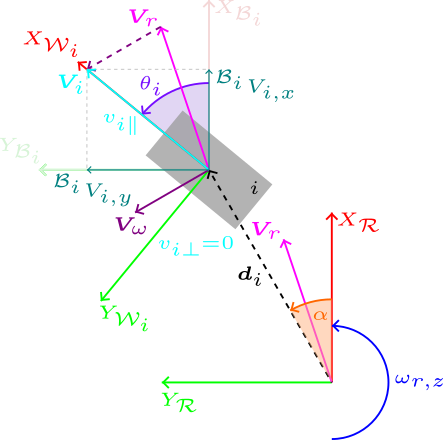
\includegraphics[width=0.8\linewidth]{images/three_swerve_drive_steerable_wheel.png}
    \caption{Rueda convencional orientable alineada con su vector de velocidad \(\vect{V}_i\) mediante una rotación de ángulo \(\theta_i\) respecto de su SC base \(\frameBi\). La dirección de rodadura queda definida por el eje \(X_{\frameWi}\) del SC fijo a la rueda \(i\), \(\frameWi\).}
    \label{fig2:tsd-steerable-wheel}
\end{figure}

Pasos para calcular la cinemática inversa de un robot con base three swerve drive:

\begin{itemize}
    \item Conocido el vector de velocidad del chasis \({}^\frameR \vect{V}_r\), se obtiene la velocidad de cada rueda \(i\) en su SC base \(\frameBi\), \({}^{\frameBi}\vect{V}_i\), aplicando la transformación de coordenadas de la ecuación \ref{eq:wheel-constraints-final}.
    \item Se calcula el ángulo de orientación \(\theta_i\) que debe adoptar cada rueda \(i\) para alinear su dirección de rodadura con el vector de velocidad \({}^{\frameBi} \vect{V}_i\) mediante la función \(\arctan2\).
          \begin{equation}
              \theta_i = \arctan2({}^{\frameBi}V_{i,y}, {}^{\frameBi}V_{i,x})
              \label{eq:tsd-inverse-kinematics-angle}
          \end{equation}
    \item Se calcula la velocidad angular de cada rueda \(i\) a partir de la expresión \ref{eq:tsd-v_parallel}.
          \begin{equation}
              \omega_i = \frac{v_{i\parallel}}{r} = \frac{\|{}^{\frameBi} \vect{V}_i\|}{r} = \frac{\sqrt{{}^{\frameBi}V_{i,x}^2 + {}^{\frameBi}V_{i,y}^2}}{r}
              \label{eq:tsd-inverse-kinematics-angular-speed}
          \end{equation}
\end{itemize}

\begin{figure}[H]
    \centering
    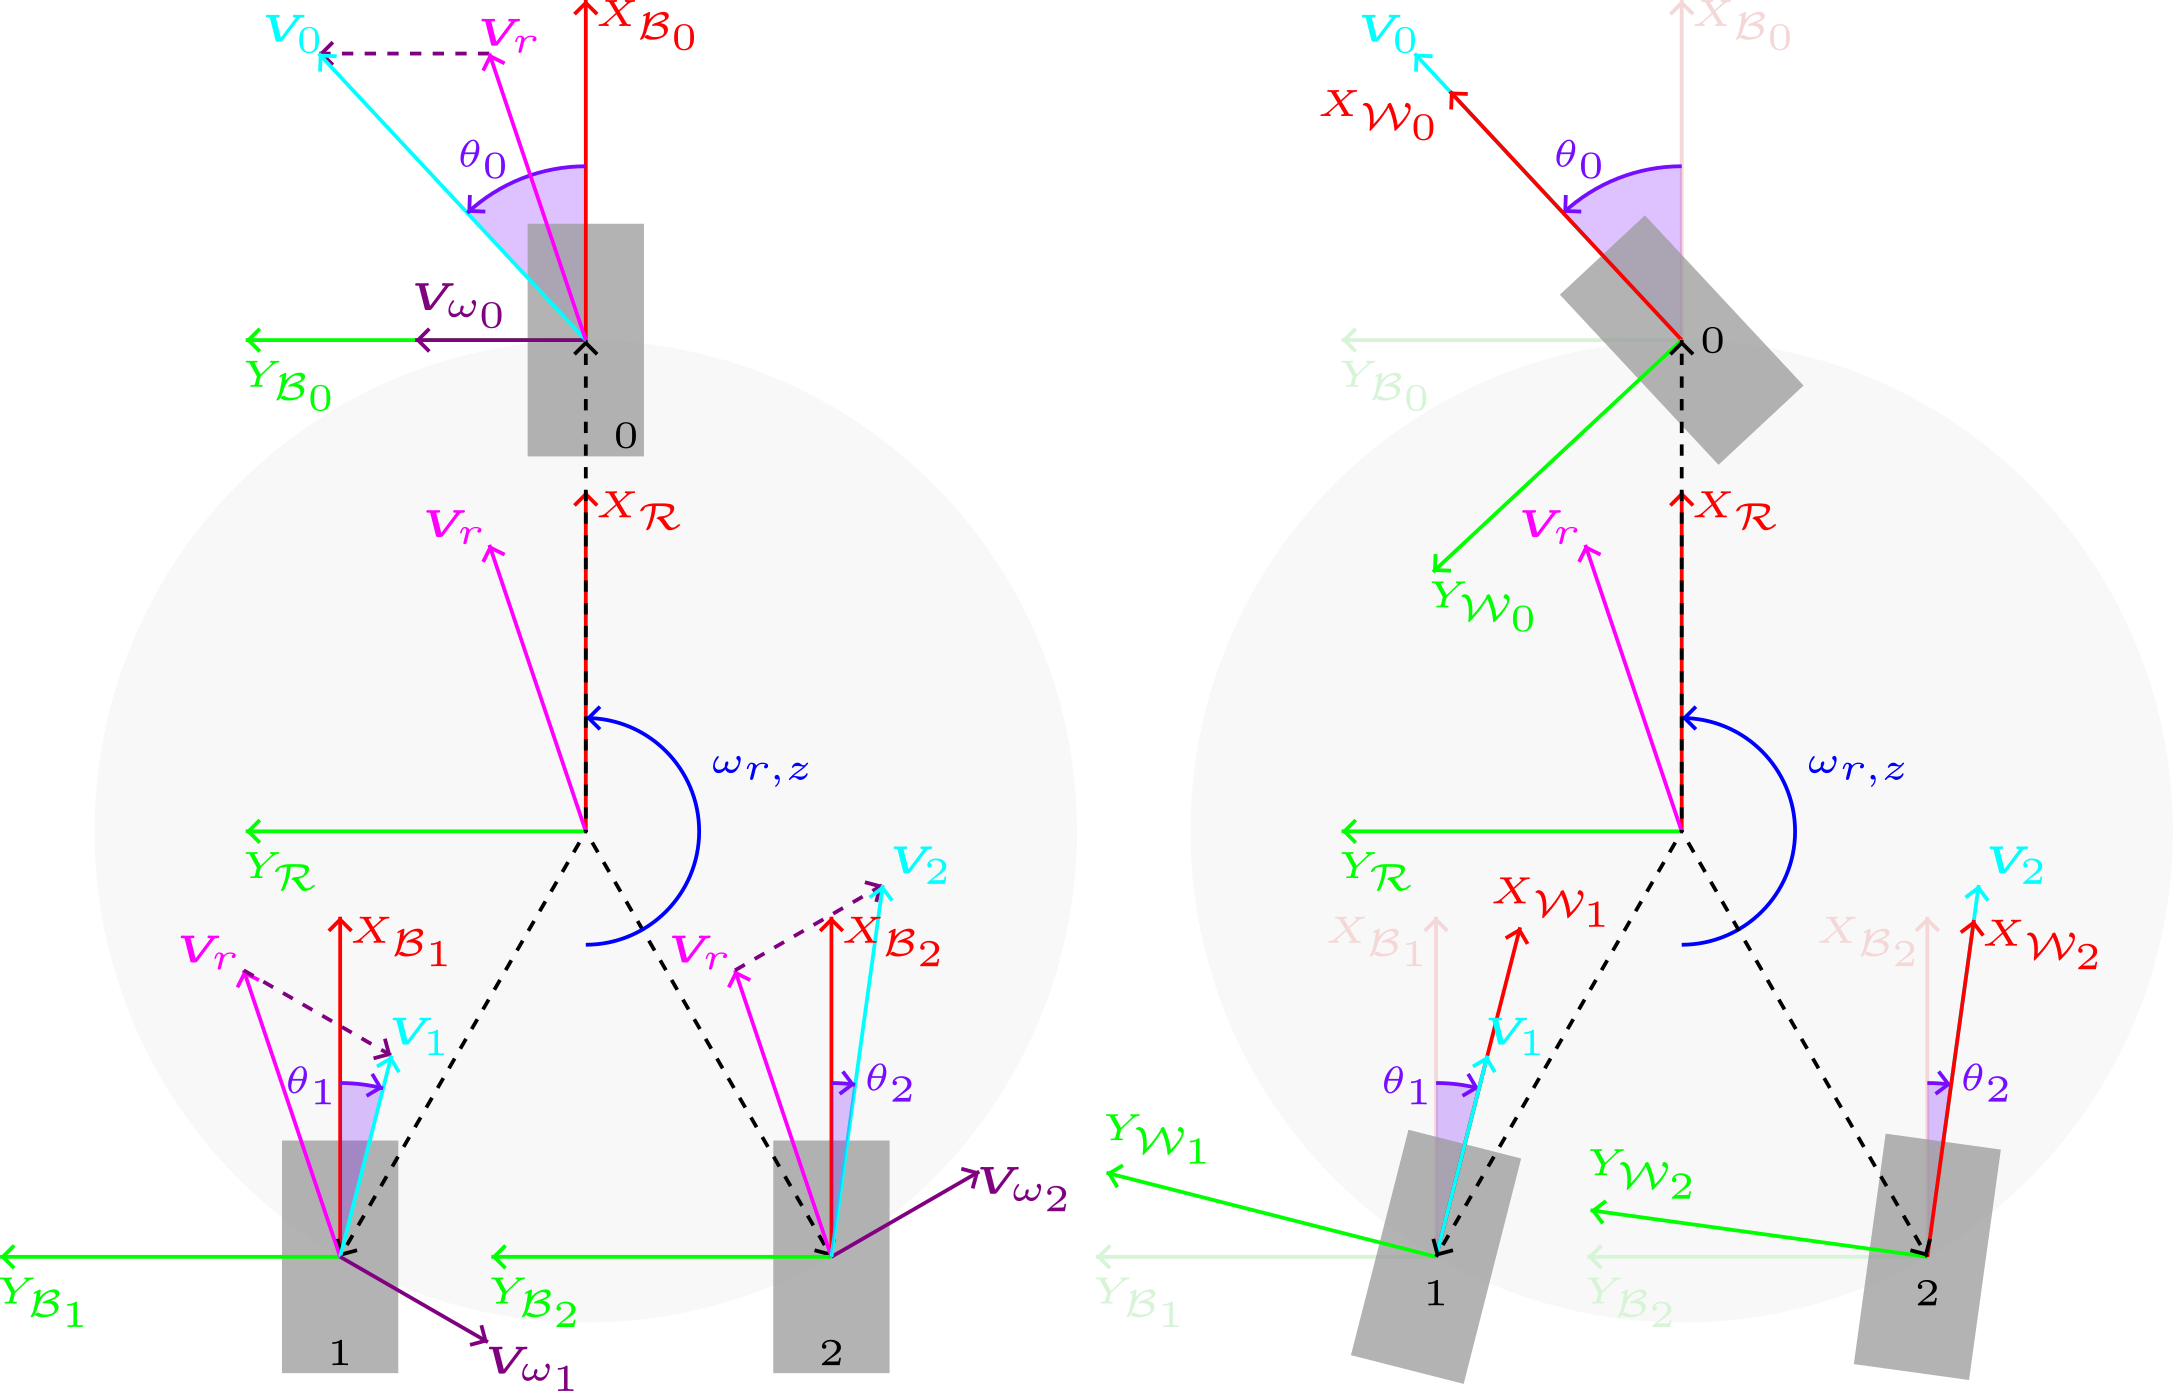
\includegraphics[width=1.0\linewidth]{images/three_swerve_drive_inverted_y_inverse_kinematics.png}
    \caption{Configuración Y-invertida. Izquierda: Cálculo del vector velocidad de cada rueda, \(\vect{V}_i\). Derecha: Orientación final que cada rueda debe adoptar (\(\theta_i\)) para alinear su dirección de rodadura con el vector de velocidad \(\vect{V}_i\).}
    \label{fig2:tsd-inverted-y-inverse-kinematics}
\end{figure}

\begin{figure}[H]
    \centering
    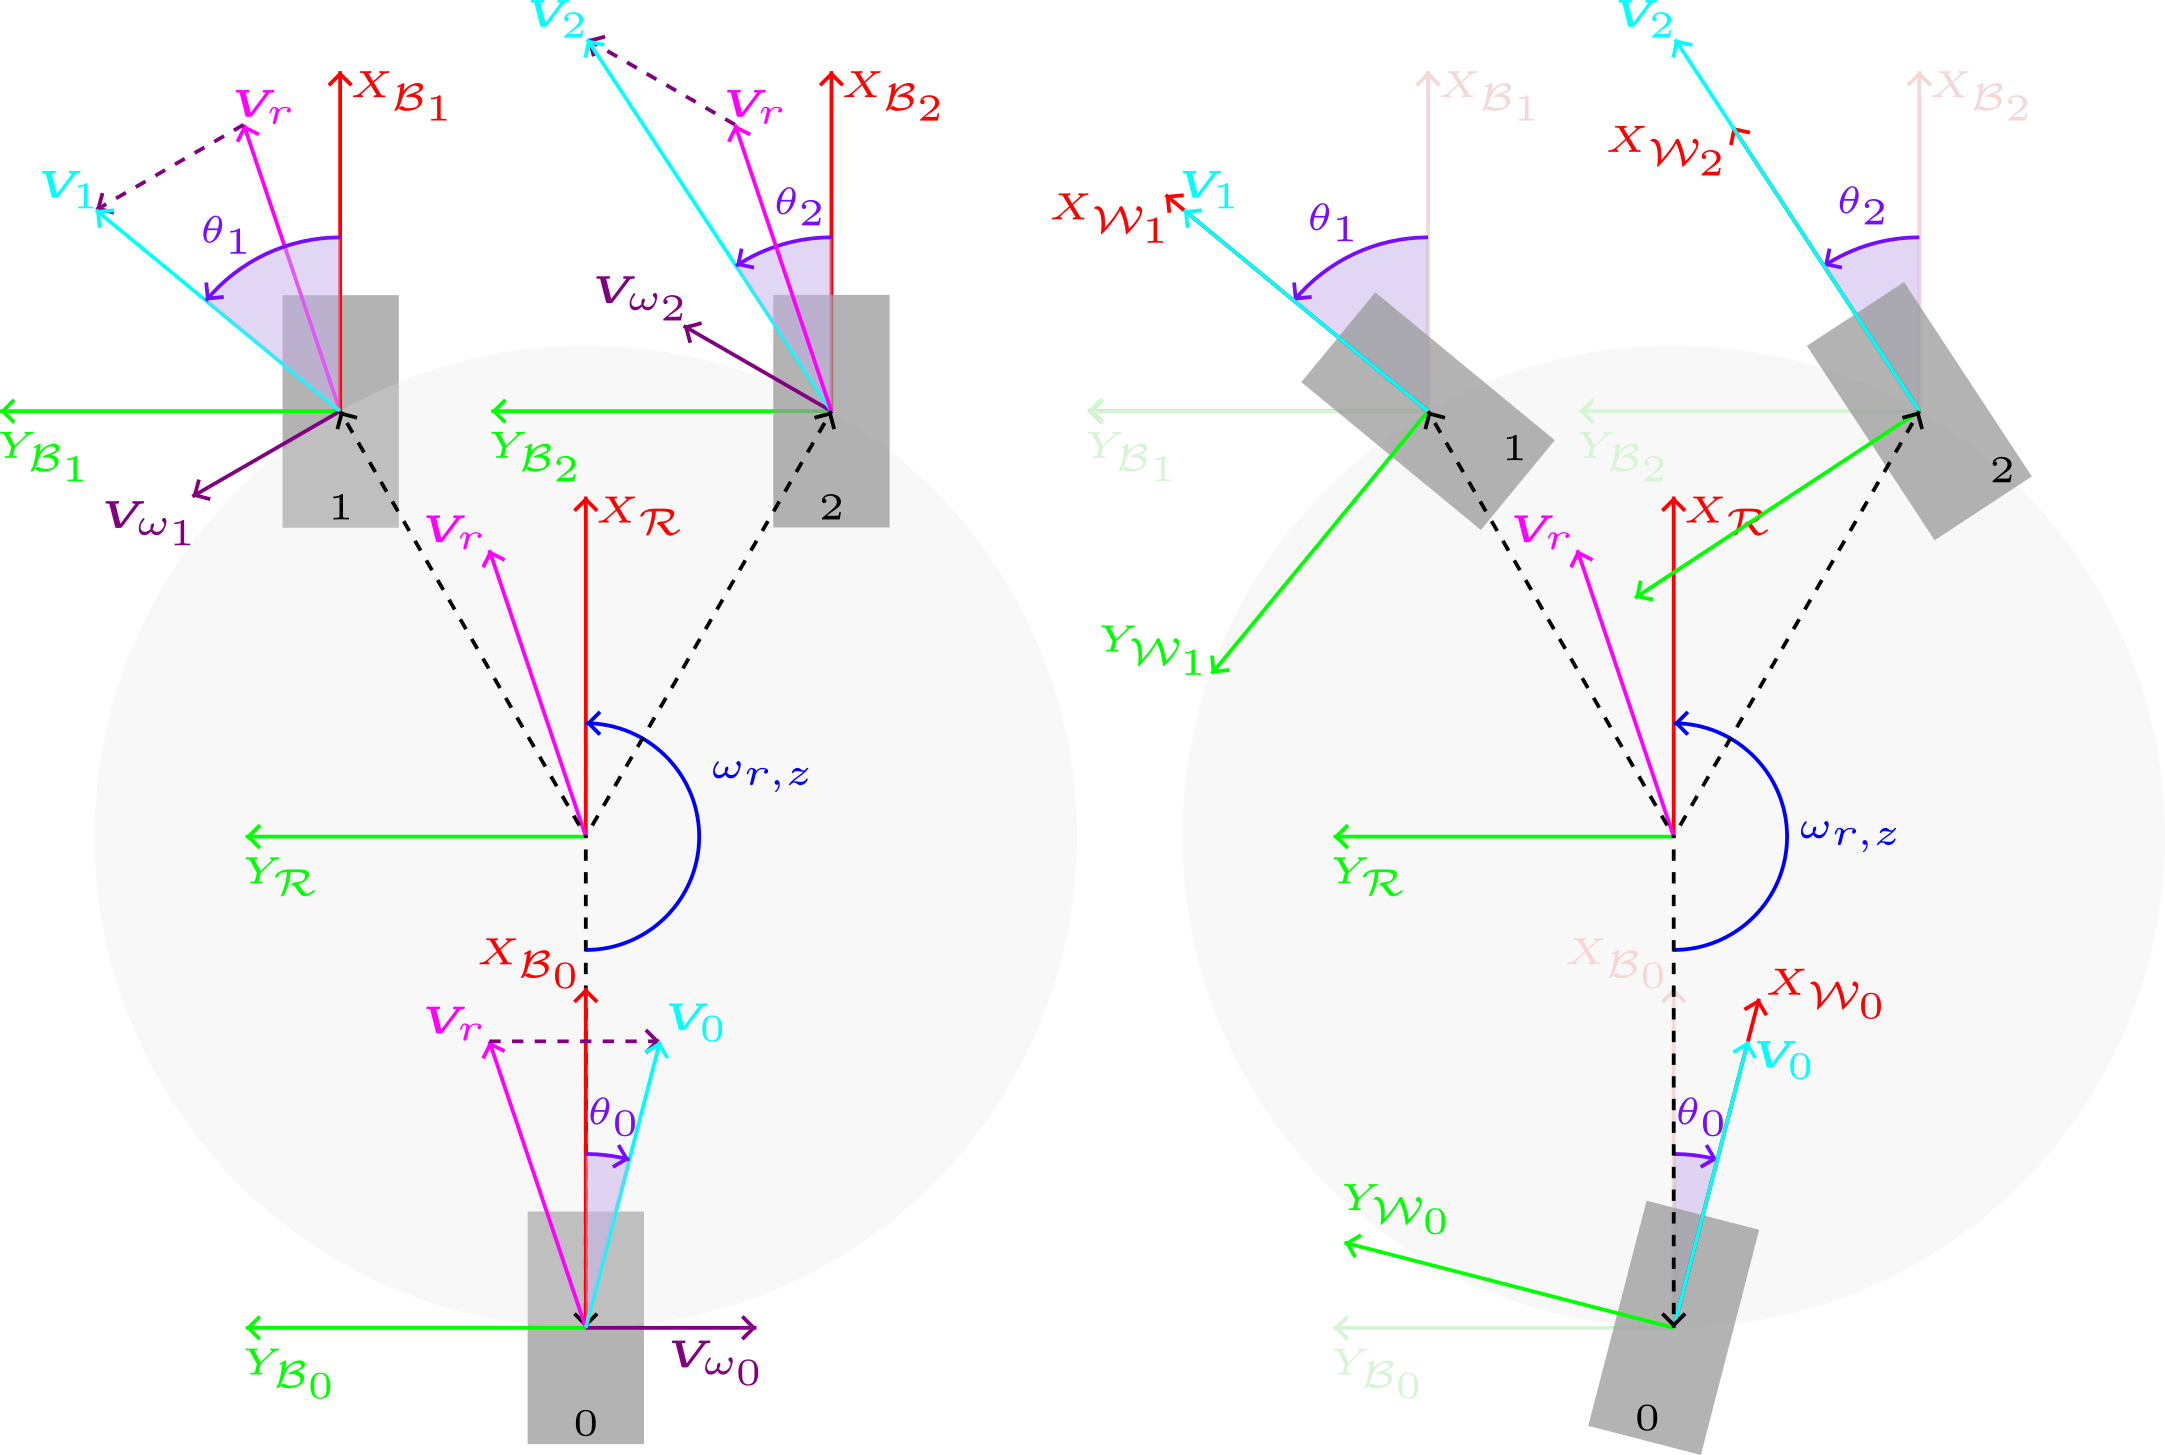
\includegraphics[width=1.0\linewidth]{images/three_swerve_drive_y_inverse_kinematics.png}
    \caption{Configuración Y. Izquierda: Cálculo del vector velocidad de cada rueda, \(\vect{V}_i\). Derecha: Orientación final que cada rueda debe adoptar (\(\theta_i\)) para alinear su dirección de rodadura con el vector de velocidad \(\vect{V}_i\).}
    \label{fig2:tsd-y-inverse-kinematics}
\end{figure}

\subsection{Cinemática directa del three swerve}

Conocidos el ángulo de orientación \(\theta_i\) y la velocidad angular \(\omega_i\) de cada rueda \(i\), se ejecutan los pasos siguientes para calcular la cinemática directa de un robot con base three swerve drive:

\begin{itemize}
    \item Calcular el vector \(\mathbf{b} = [{}^{\frameBZero}V_{0,x}, {}^{\frameBZero}V_{0,y}, \ldots, {}^{\frameBNMinusOne}V_{N-1,x}, {}^{\frameBNMinusOne}V_{N-1,y}]^{\trans}\).\\
          Donde:
          \begin{equation}
              \begin{aligned}
                  {}^{\frameBi}V_{i,x} & = \|{}^{\frameBi}\vect{V}_i\| \cos\theta_i = v_{i\parallel}\cos\theta_i = r\omega_i\cos\theta_i \\
                  {}^{\frameBi}V_{i,y} & = \|{}^{\frameBi}\vect{V}_i\| \sin\theta_i = v_{i\parallel}\sin\theta_i = r\omega_i\sin\theta_i
              \end{aligned}
          \end{equation}
    \item Resolver el sistema lineal \(A\mathbf{x} = \mathbf{b}\) mediante la pseudoinversa de \(A\), \(A^+\), como se explicó en la Sección \ref{sec:general-considerations}, para obtener la velocidad del chasis \(\mathbf{x} = [{}^\frameR V_{r,x}, {}^\frameR V_{r,y}, \omega_{r,z}]^{\trans}\). Obviamente, usando la matriz \(A\) correspondiente a la configuración de ruedas considerada, Y-invertida o Y.
\end{itemize}

\end{document}
